\chapter{Results}
\label{s_results}

This chapter presents the results of the path planning framework developed in this work. 
It reports representative trajectories between selected vertiports in the Hamburg scenario (Sec.~\ref{sec:scenario}), 
the associated kinematic profiles (true airspeed, turn rate, altitude, bank angle), 
geometric properties of the paths, and computational performance for planning and trajectory generation 
(Secs.~\ref{sec:astar_global} and \ref{s_traj_generation}). 
A dedicated section (Sec.~\ref{sec:results_conflicts}) demonstrates conflict detection outcomes using NDMap (method in Sec.~\ref{sec:ndmap}).

\medskip
\noindent
All trajectories and profiles shown in this chapter are \emph{planned (reference) 4D trajectories} produced by the pipeline, i.e., the intended paths to be followed by the aircraft; they are not simulation runs.

\section{Experimental Setup}
\label{sec:results_setup}

\subsection{Scenario and Data}
The experiments are conducted on the Hamburg vertiport network described in Sec.~\ref{sec:scenario}, 
with corridors modeled as undirected edges at a constant altitude layer of \SI{200}{m} AGL and width \SI{20}{m}. 
Nodes correspond to vertiports (averaged pad coordinates); edges are weighted by geodesic distance.

\subsection{Planner and Generator Configuration}
\begin{itemize}
  \item \textbf{Global planner:} A* on the undirected corridor graph (Sec.~\ref{sec:astar_global}), with Haversine heuristic \(h(n)\) and evaluation function \(f(n)=g(n)+h(n)\).
  \item \textbf{Trajectory generator:} CFMS-based 4D trajectory synthesis (Sec.~\ref{s_traj_generation}) with cruise height \(H_c=\SI{200}{m}\) (AGL), speed profile \((V_{\text{takeoff}}, V_{\text{transition}}, V_{\text{cruise}}, V_{\text{approach}})\).
\end{itemize}

\subsection{Evaluation Metrics}
The following metrics are reported for each run:
\begin{itemize}
  \item \textbf{Path geometry:} number of legs, total length \(L\) (km).
  \item \textbf{Timing:} total flight time \(T\) (s), average TAS.
  \item \textbf{Kinematics:} TAS profile, altitude compliance w.r.t.\ \(H_c\), peak bank angle \(\max \phi\), peak turn rate \(\max \dot{\psi}\).
  \item \textbf{Compute:} A* runtime and trajectory generation time.
\end{itemize}

\section{Case Studies: Sample Trajectories}
\label{sec:results_case_studies}

This section presents representative trajectories between selected vertiport pairs. 
For each case, \(s\) denotes the starting vertiport and \(d\) the destination.

\subsection{Representative Long-Leg Route}
\label{sec:trajA}

Trajectory A was selected as a representative case because it contains one of the longest legs in the Hamburg network. 
This results in a comparatively high total path length and flight time. 
Furthermore, the extended initial leg allows the UAM vehicle sufficient time to transition from take-off into the corridor 
network, stabilizing its climb and entering the cruise segment more gradually. 
This makes Trajectory A well-suited for evaluating the performance of the global planner and the consistency of the 
generated cruise profile.

\subsubsection*{Route Overview}
\begin{figure}[H]
  \centering
  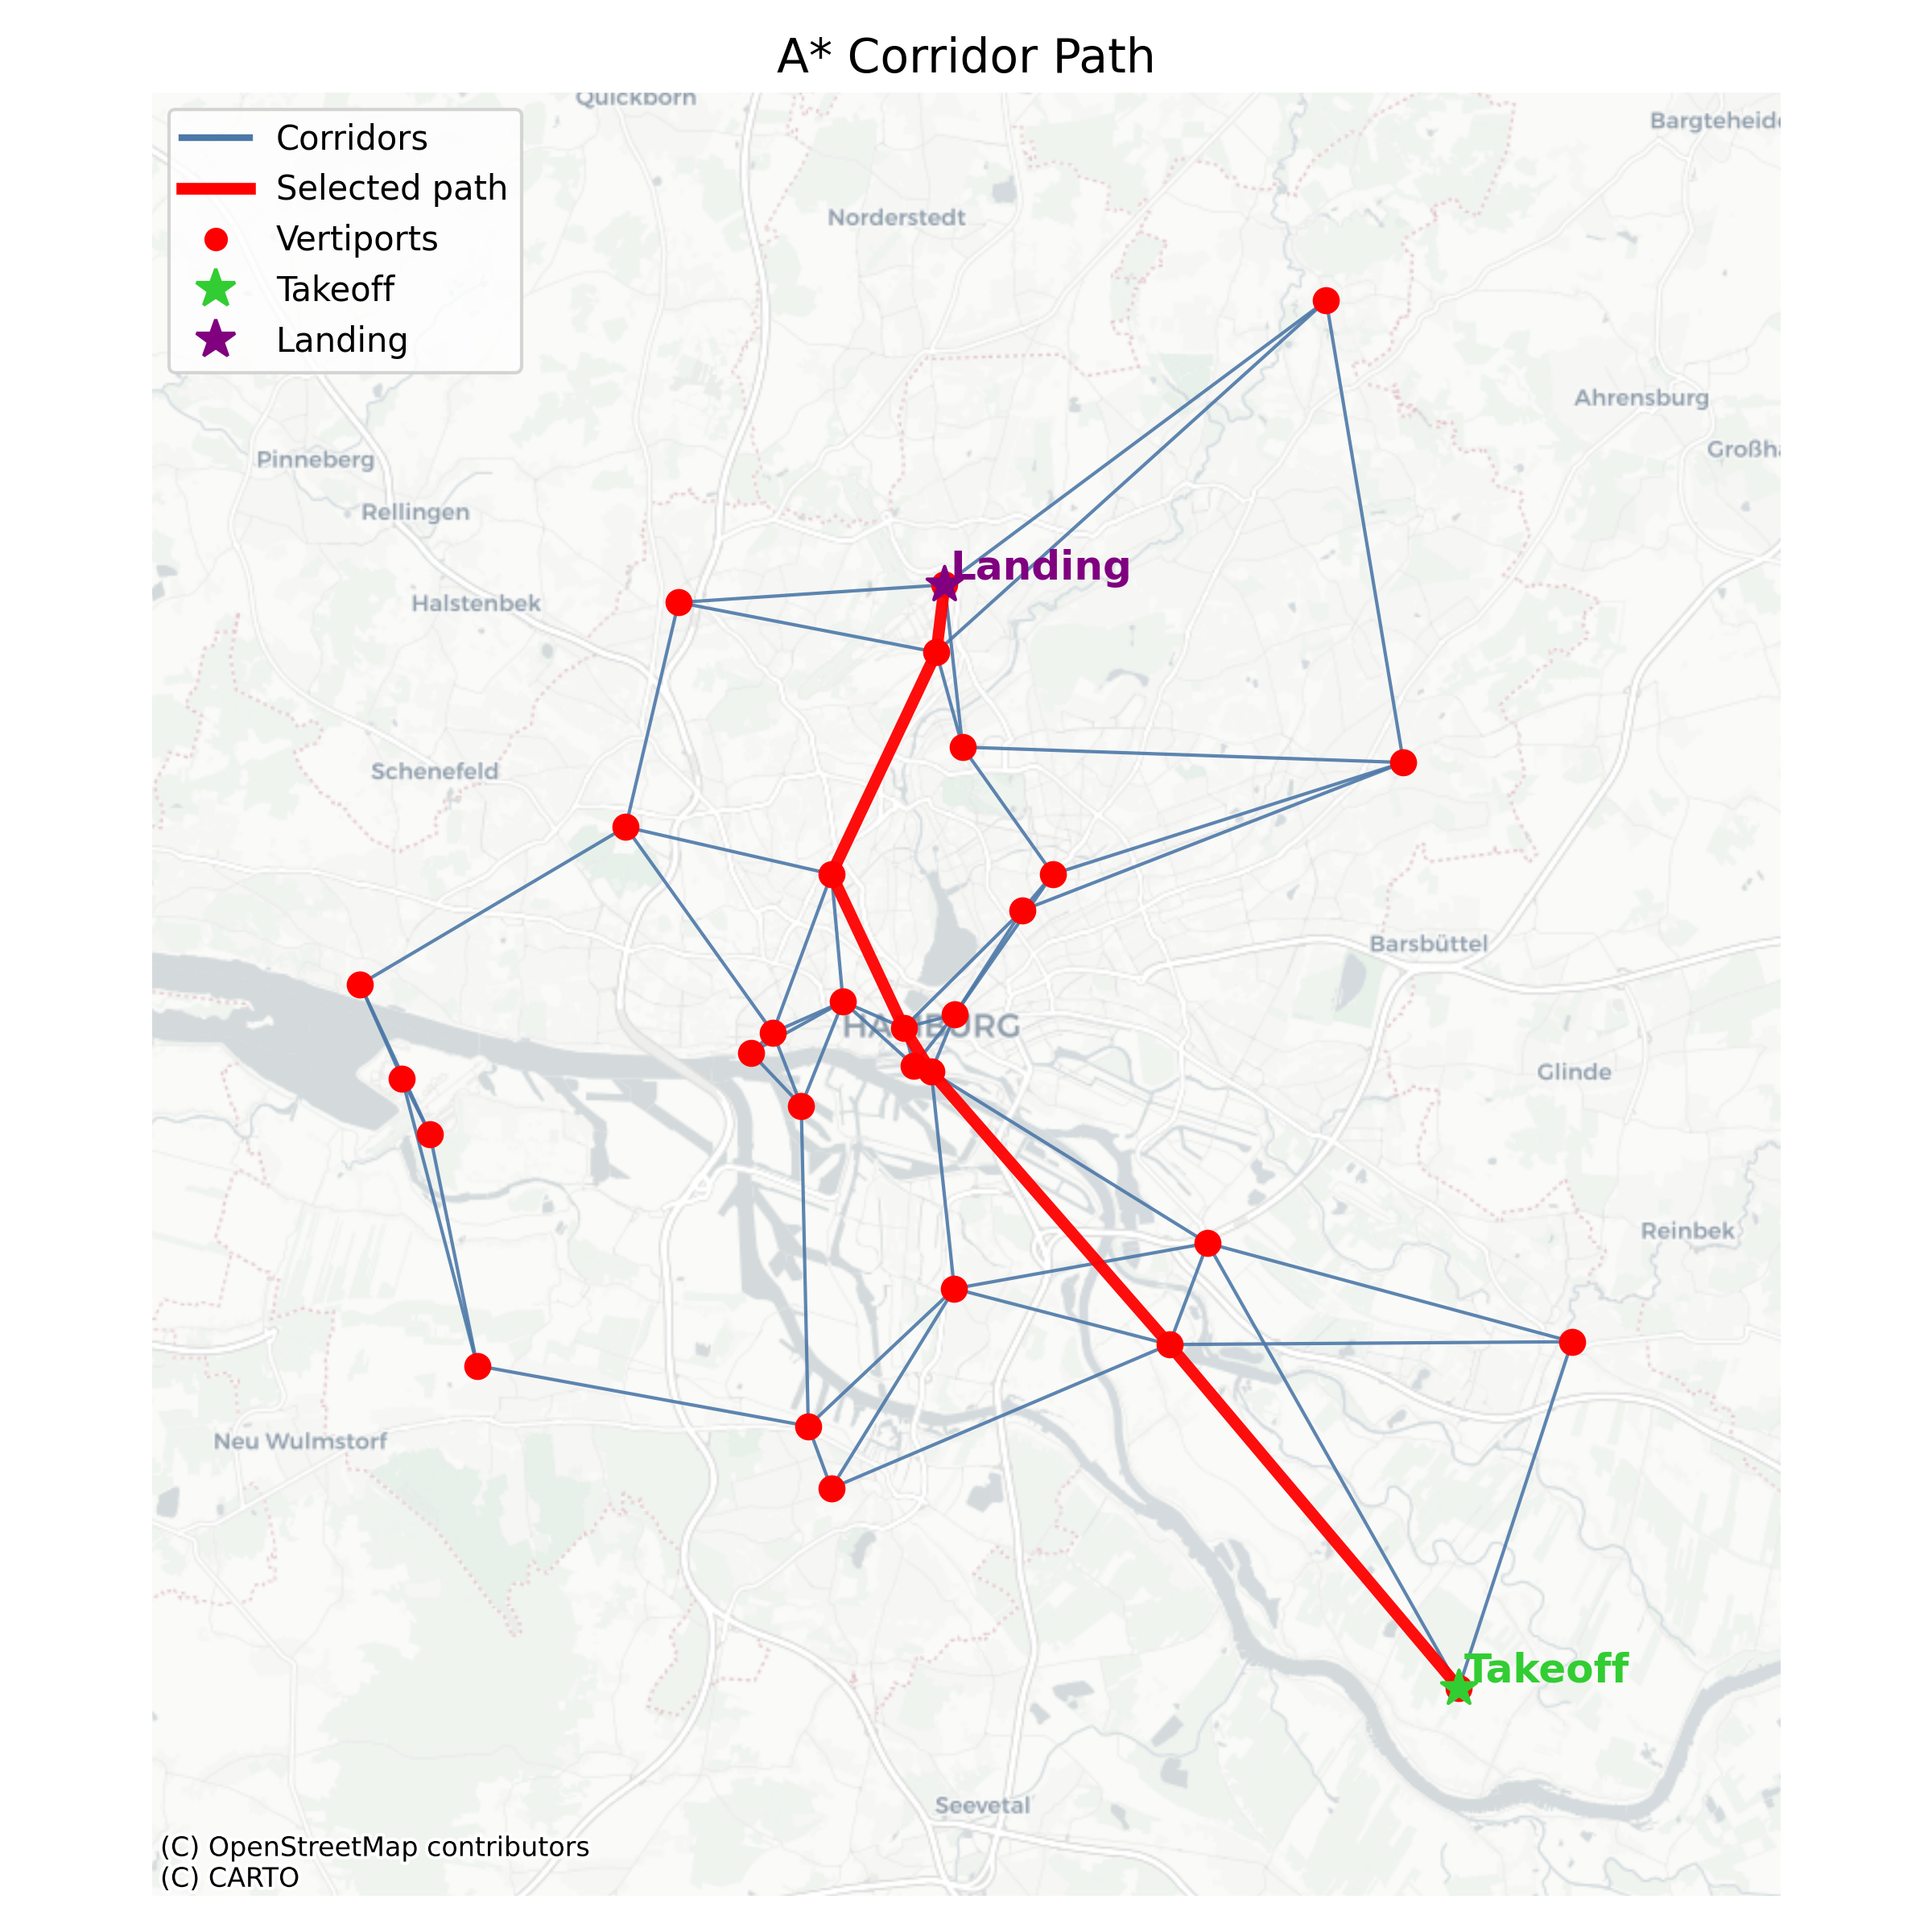
\includegraphics[width=0.6\textwidth]{results/trajectoryA_map.png}
  \caption{Planned reference trajectory (Trajectory A) from \(s\) to \(d\) over the Hamburg corridor network.}
  \label{fig:trajA_map}
\end{figure}

\subsubsection*{Front-end Visualization (Cesium)}
Figure~\ref{fig:trajA_cesium} shows the planned Trajectory~A rendered in the Cesium-based web client. 
The left view displays the full 3D corridor context of the route, while the right view 
zooms in on the departure phase to highlight the take-off and initial climb segment.

\begin{figure}[H]
  \centering
  \begin{subfigure}[t]{0.48\textwidth}
    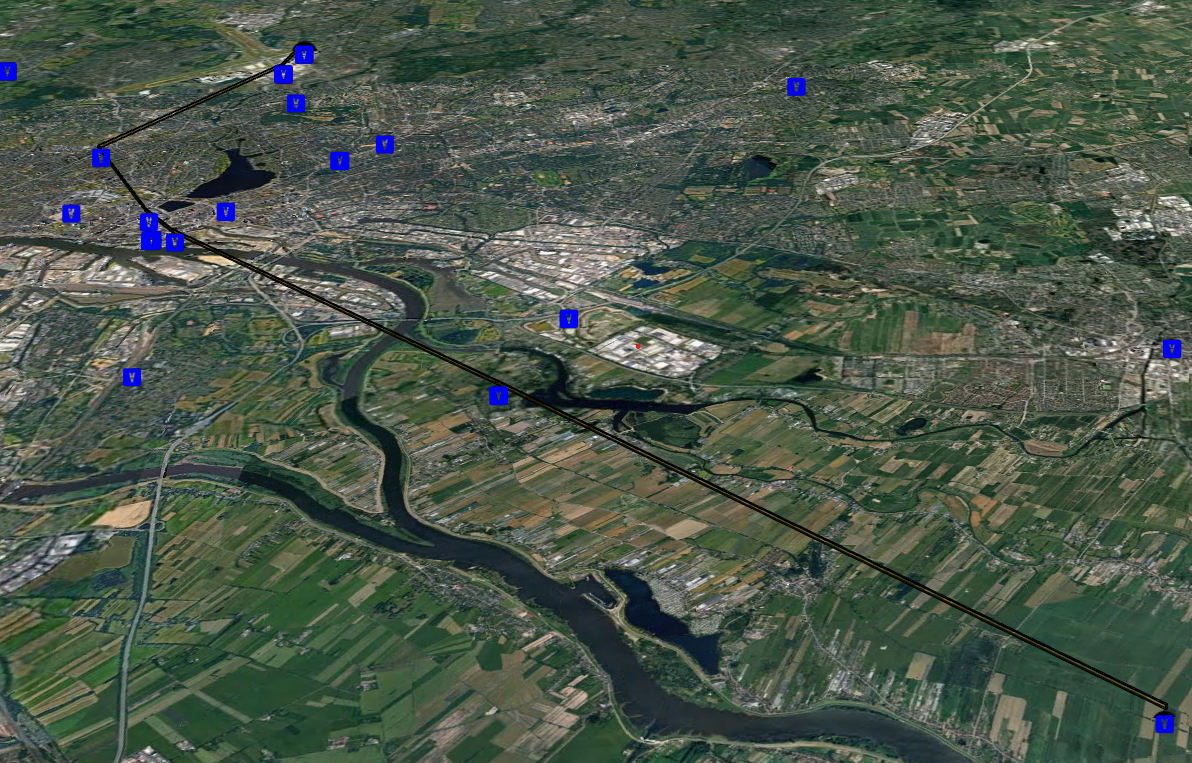
\includegraphics[width=\textwidth]{results/trajectoryA_cesium_full.png}
    \caption{Planned route (Trajectory A): full 3D corridor context.}
  \end{subfigure}
  \hfill
  \begin{subfigure}[t]{0.48\textwidth}
    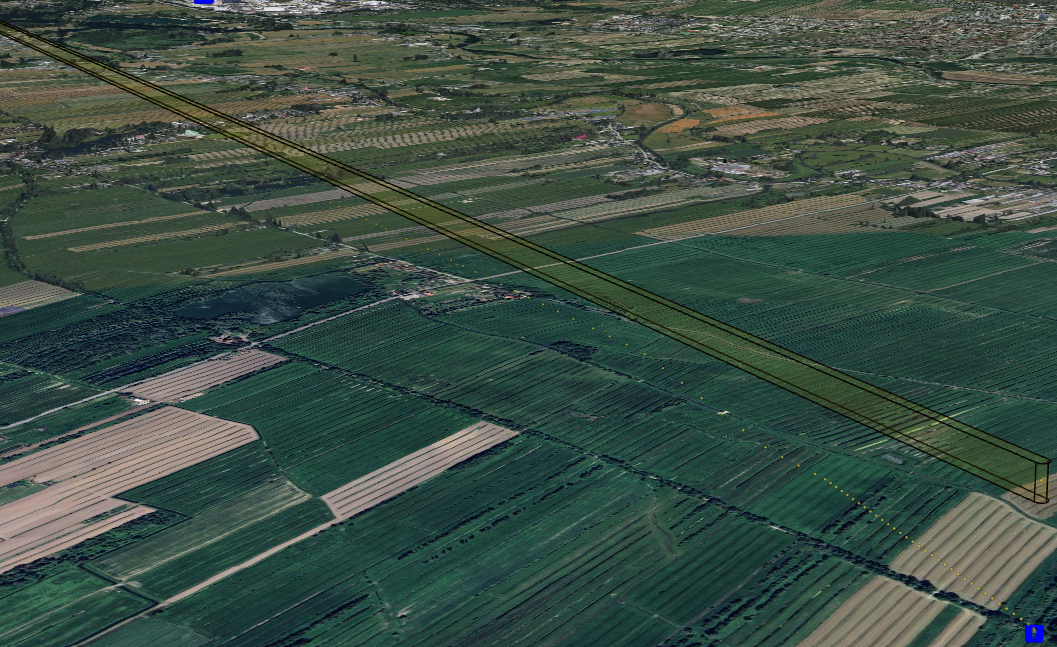
\includegraphics[width=\textwidth]{results/trajectoryA_cesium_takeoff.png}
    \caption{Planned route (Trajectory A): zoom on take-off and initial climb.}
  \end{subfigure}
  \caption{Cesium-based visualization of the planned Trajectory~A in the front end. Left: full route; right: take-off segment.}
  \label{fig:trajA_cesium}
\end{figure}

\subsubsection*{Kinematic Profiles}
\begin{figure}[H]
  \centering
  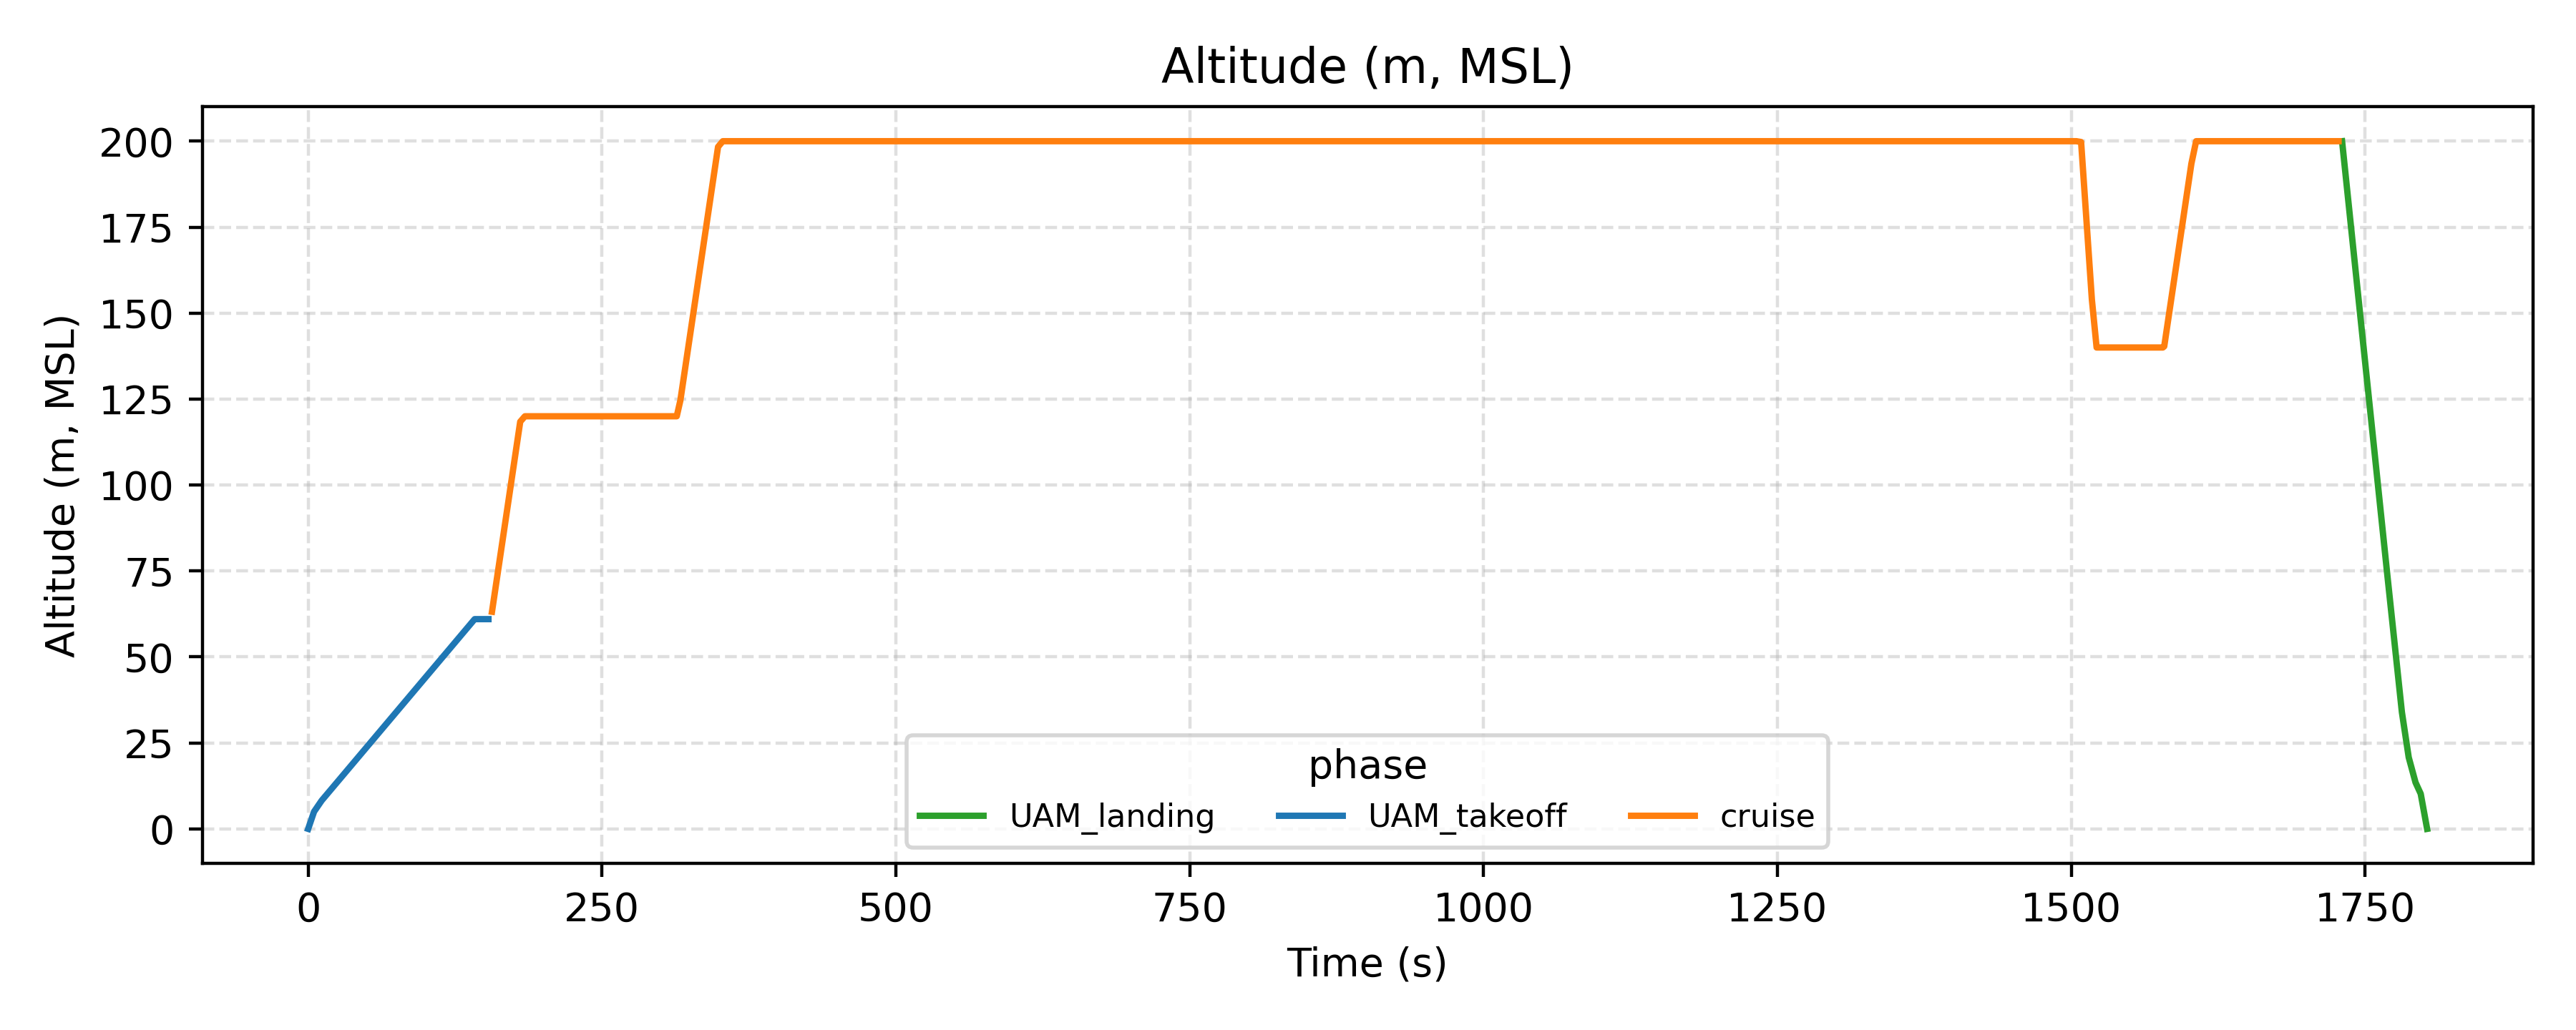
\includegraphics[width=0.86\textwidth]{results/trajectoryA_altitude.png}
  \caption{Planned altitude profile \(H(\tau)\) for Trajectory A (cruise layer near \SI{200}{m} AGL).}
  \label{fig:trajA_alt}
\end{figure}

\begin{figure}[H]
  \centering
  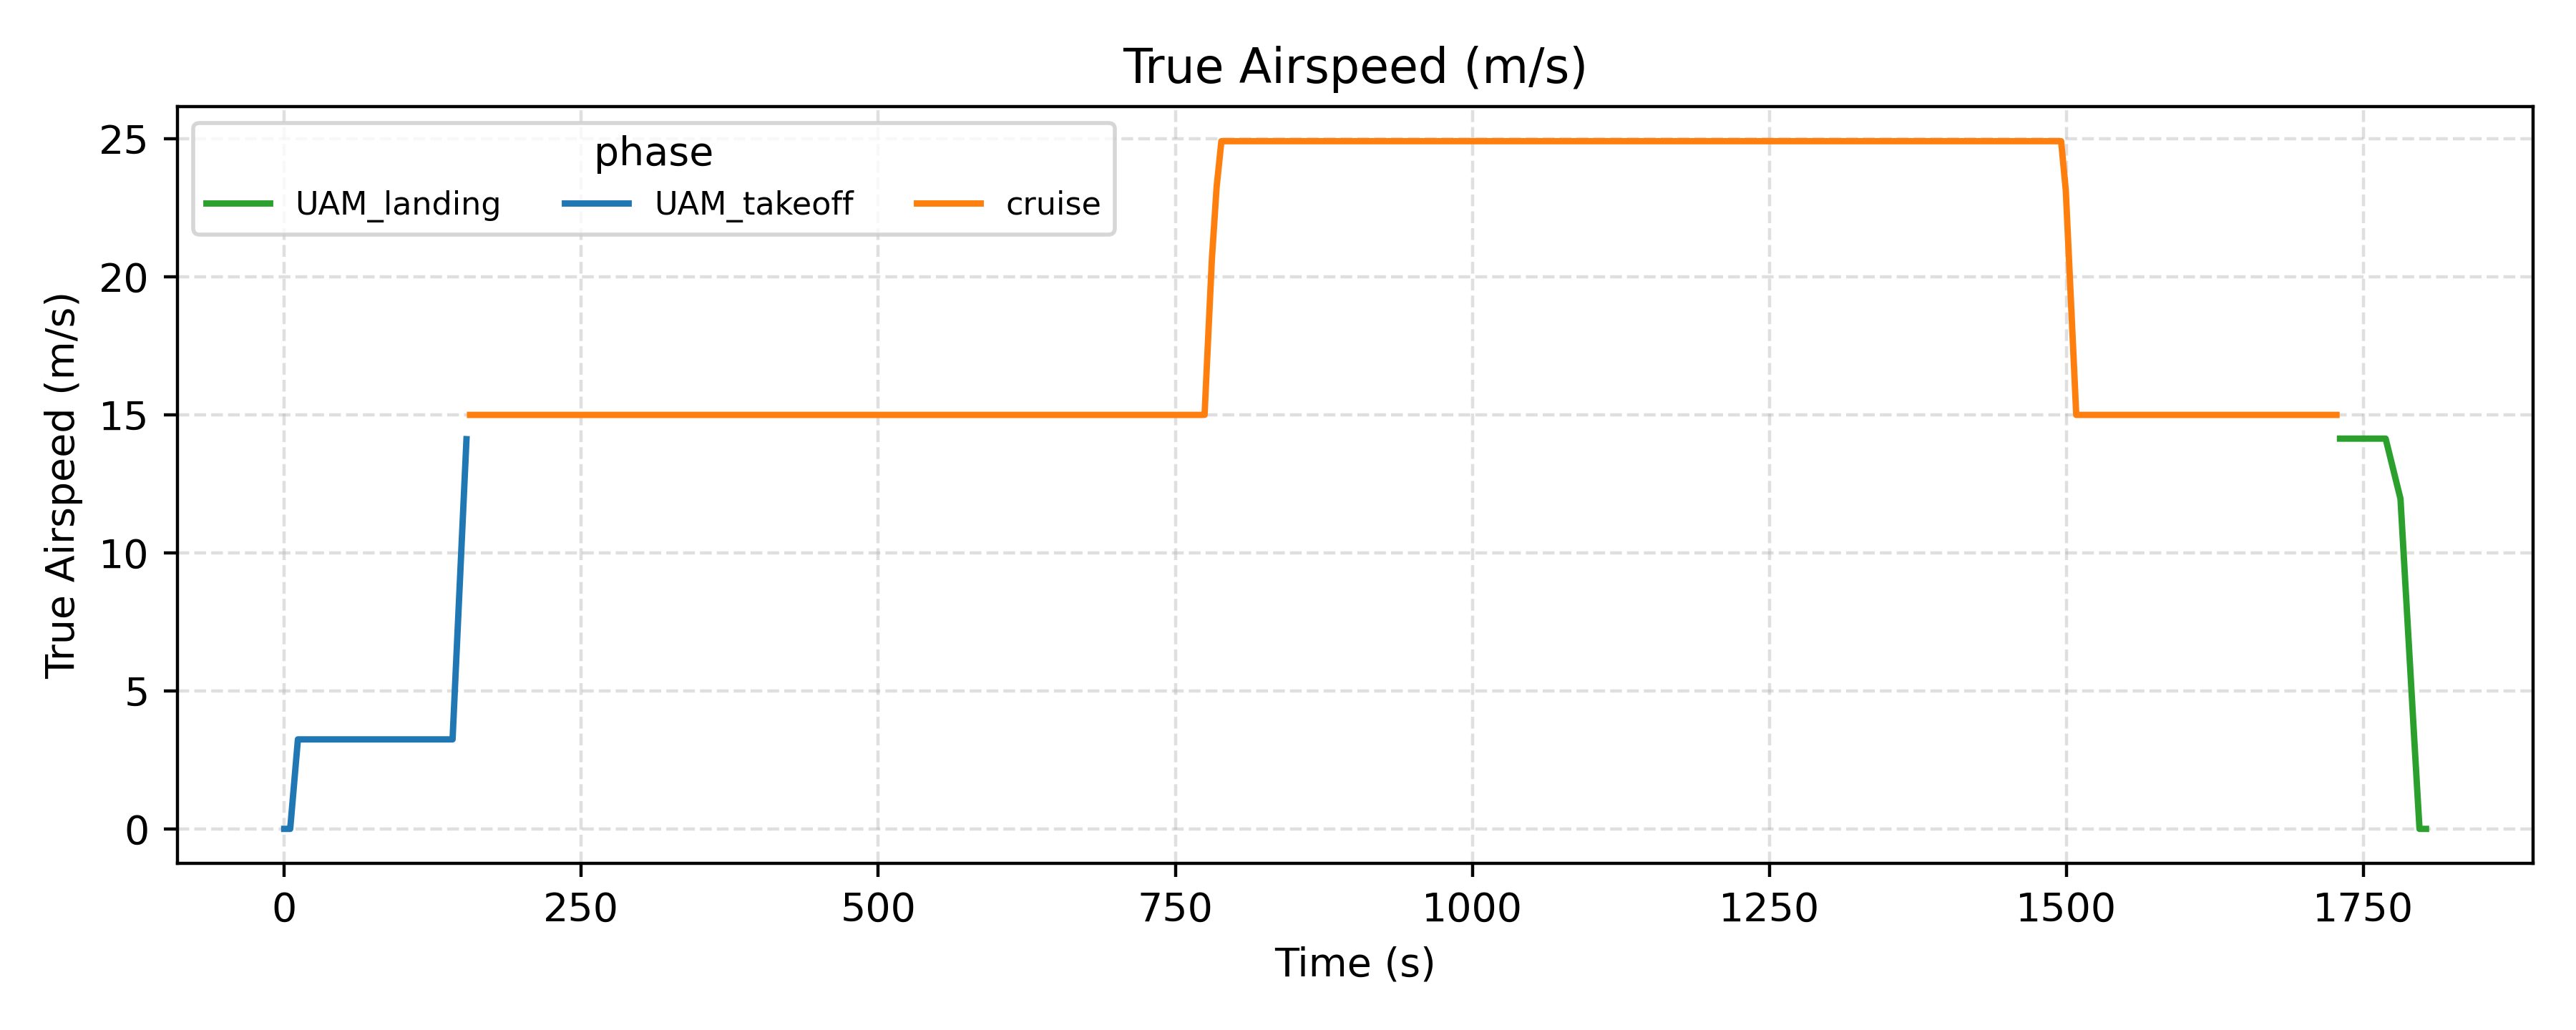
\includegraphics[width=0.86\textwidth]{results/trajectoryA_TAS.png}
  \caption{Planned true airspeed (TAS) profile for Trajectory A.}
  \label{fig:trajA_tas}
\end{figure}

\begin{figure}[H]
  \centering
  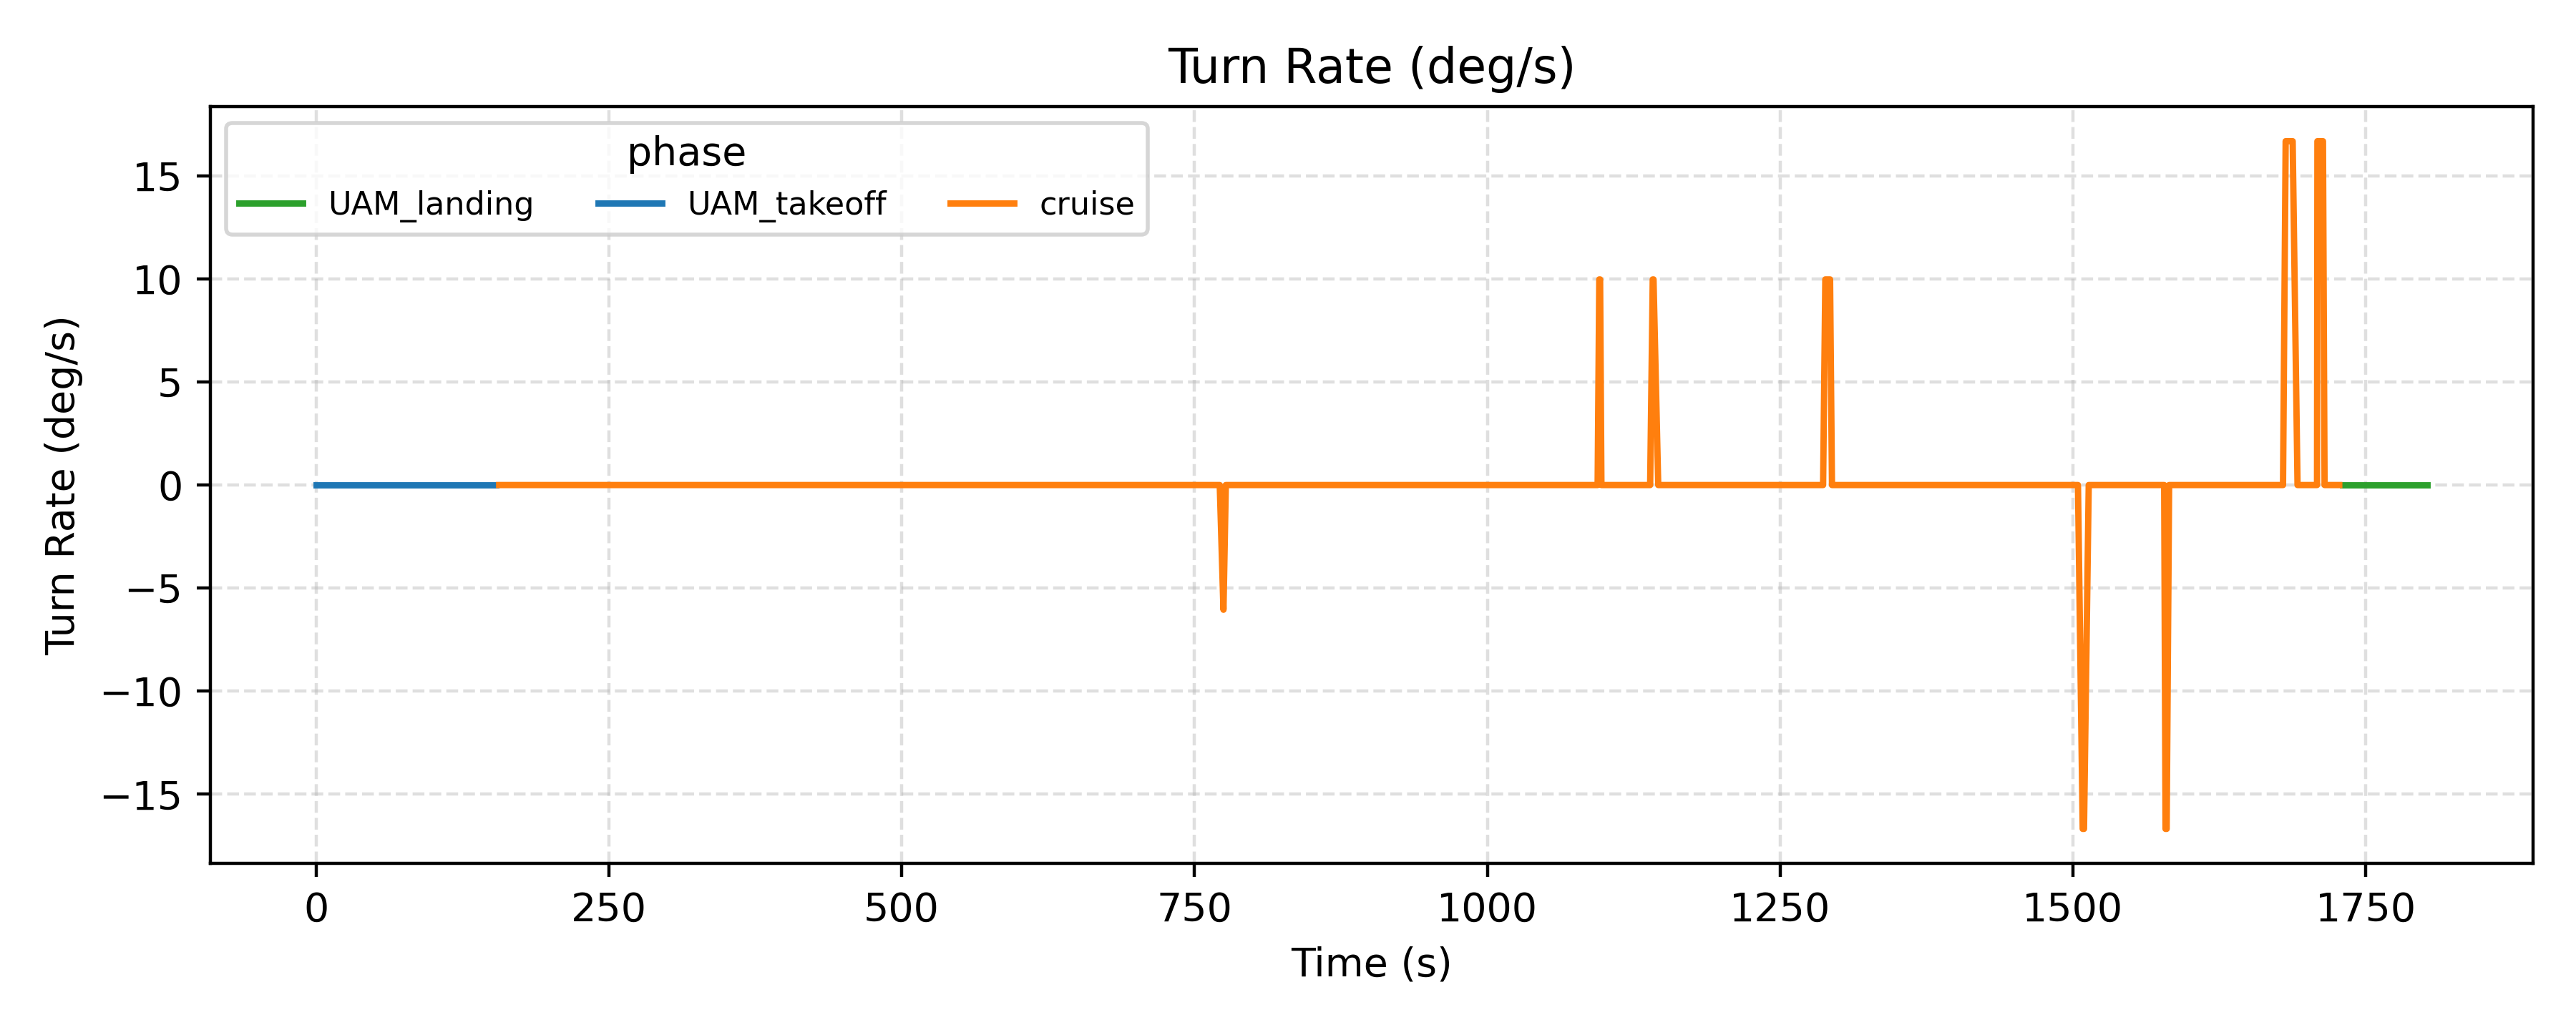
\includegraphics[width=0.86\textwidth]{results/trajectoryA_turn.png}
  \caption{Planned turn-rate profile \(\dot{\psi}(\tau)\) for Trajectory A (deg/s).}
  \label{fig:trajA_turn}
\end{figure}

\begin{figure}[H]
  \centering
  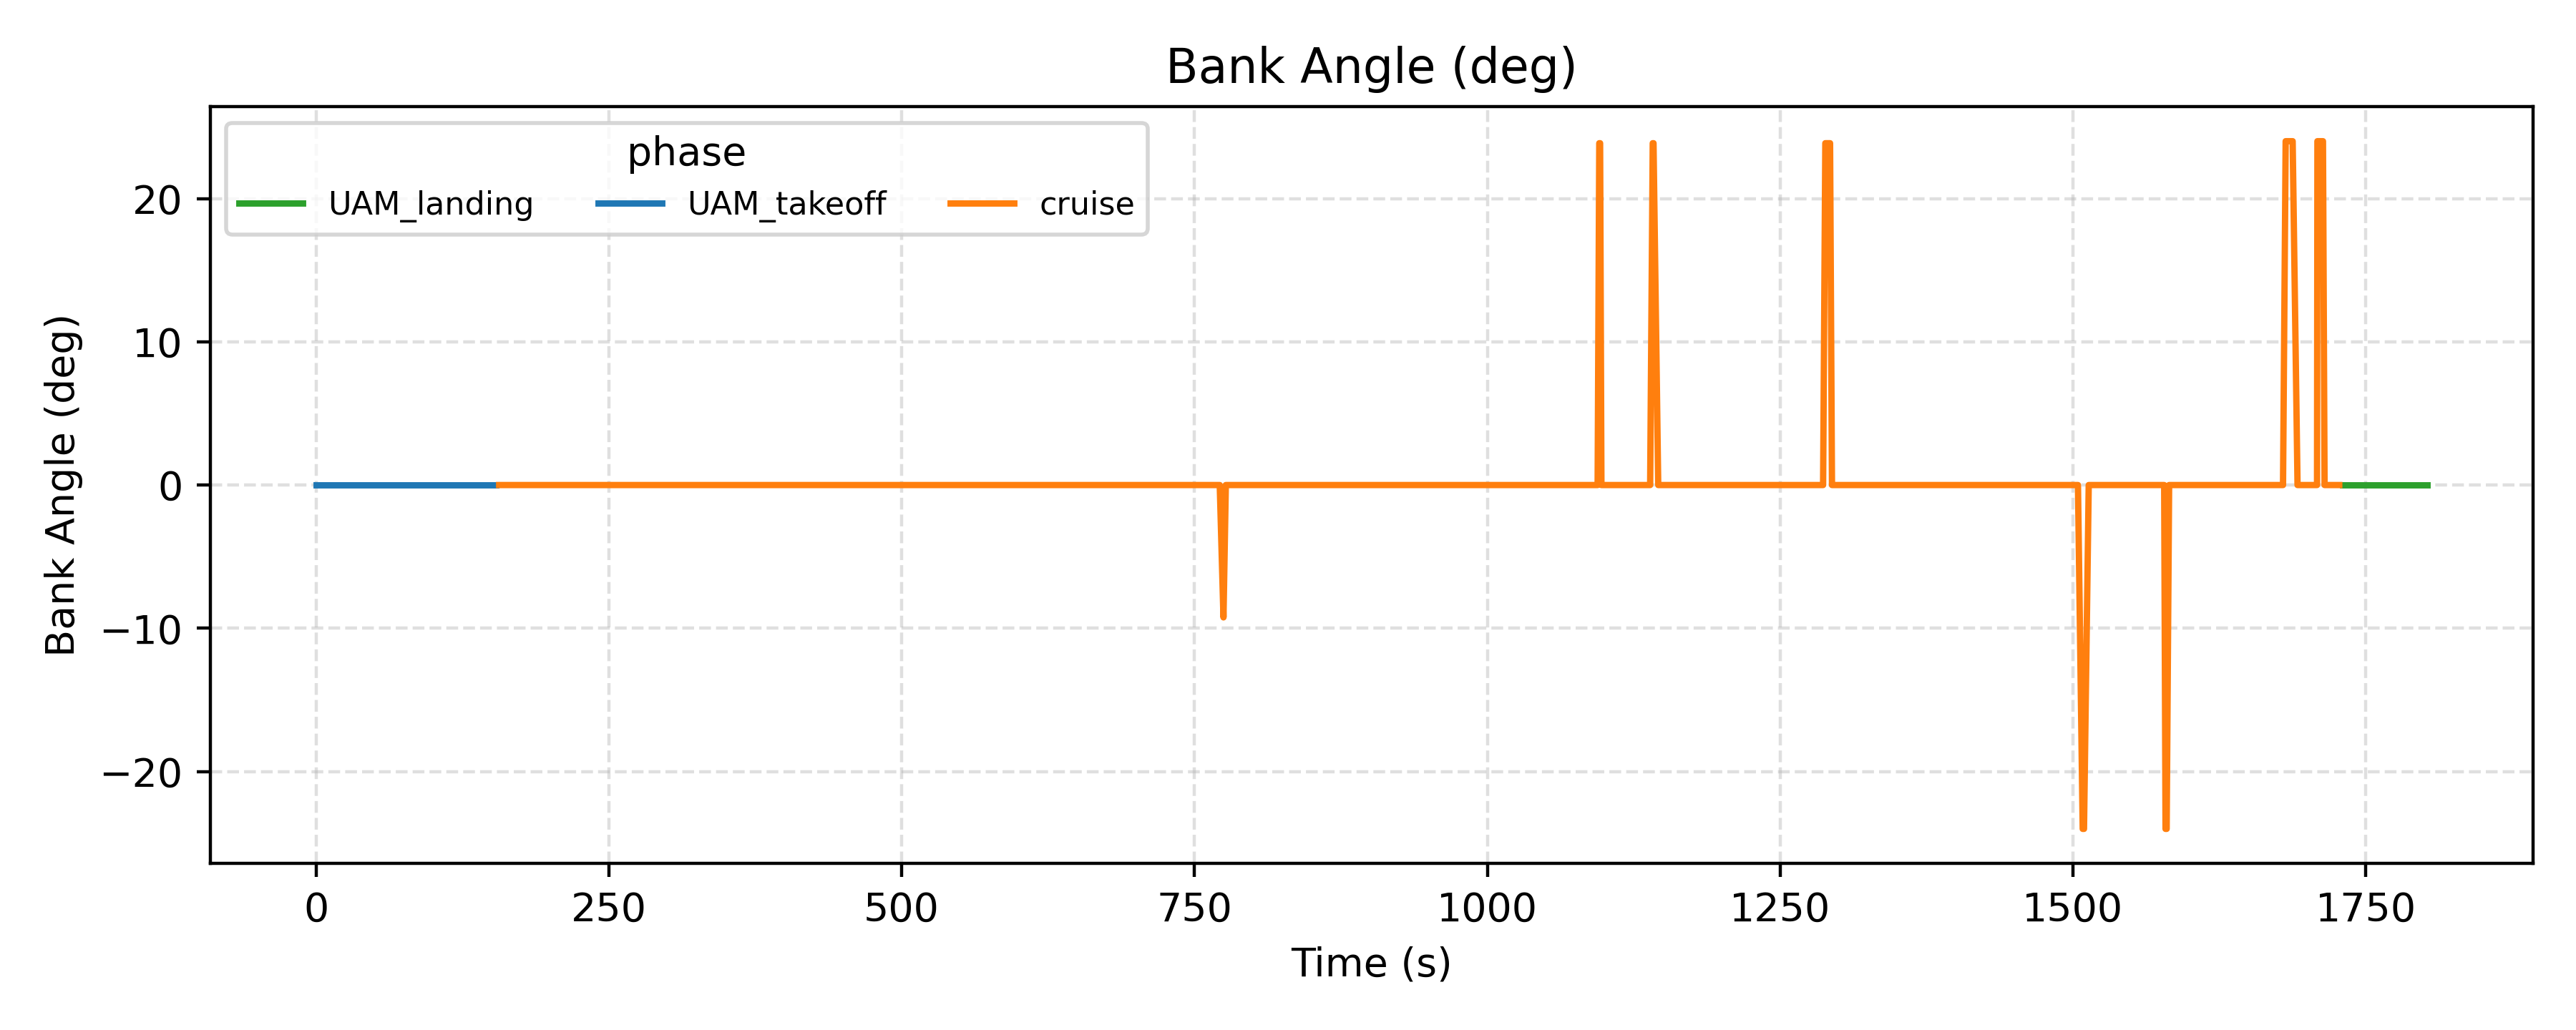
\includegraphics[width=0.86\textwidth]{results/trajectoryA_bank.png}
  \caption{Planned bank-angle profile $\phi(\tau)$ for Trajectory A (deg).}
  \label{fig:trajA_bank}
\end{figure}

\paragraph{Interpretation of bank angle and turn-rate profiles (CFMS).}
At each turn waypoint, the inbound and outbound ground tracks define the required course change \(\Delta\chi\) and the turn direction. 
CFMS then synthesizes a dynamically feasible turn using the aircraft performance limits (maximum load factor and bank-rate limit) at the current \emph{groundspeed} \(V_g\) (speed over ground, i.e., the magnitude of the ground-relative velocity vector) \cite{morscheck2021cfms}. 
The constructed turn has three phases: bank-up, constant-bank arc, and bank-down. A bank-rate bound \(\dot\phi_{\max}\) shapes the transients; if the transients would exceed the geometric corner, CFMS reduces the allowable bank to fit the fillet.

The bank ceiling is set by the maximum load factor \(n_{\max}\) under coordinated-turn assumptions:
\begin{equation}
  \phi_{\max} \;=\; \arccos\!\left(\frac{1}{n_{\max}}\right).
\end{equation}
The instantaneous turn rate follows coordinated-turn kinematics:
\begin{equation}
  \dot\psi(t) \;=\; \frac{g\,\tan\!\big(\phi(t)\big)}{V_g(t)}\,,
\end{equation}
so, for a given \(V_g\), the largest achievable turn rate is
\begin{equation}
  \dot\psi_{\max} \;=\; \frac{g\,\tan(\phi_{\max})}{V_g}\,.
\end{equation}

\noindent\textit{Consistency check for reported peaks.}
Using the study’s typical value \(n_{\max}=1.1\) (small UAS),
\begin{equation}
  \phi_{\max} \;\approx\; \arccos\!\left(\frac{1}{1.1}\right) \;\approx\; 24.6^{\circ},
\end{equation}
which is consistent with the observed \(\max \phi \approx 24.0^{\circ}\).
At a representative transitional groundspeed \(V_g \approx 15~\mathrm{m/s}\),
\begin{equation}
    \begin{aligned}
      \dot\psi_{\max} 
      &\;\approx\; \frac{9.81\,\tan(24^{\circ})}{15}\;\; \mathrm{rad/s} \\
      &\;\approx\; 0.29~\mathrm{rad/s} \;\approx\; 16.7^{\circ}\!/\mathrm{s},
    \end{aligned}  
\end{equation}
matching the reported \(\max \dot\psi \approx 16.68^{\circ}\!/\mathrm{s}\).
(When CFMS’s simplified point-to-point routine is used, a capped constant turn rate may be applied instead of the full filleted turn.)

\subsubsection*{Summary Statistics}
\begin{table}[H]
  \centering
  \caption{Summary statistics for the planned reference Trajectory A.}
  \label{tab:trajA_summary}
  \begin{tabular}{l r}
    \toprule
    Points & \num{500} \\
    Total time $T$ (s) & \num{1802.71} \\
    Total time $T$ (min) & \num{30.05} \\
    Total distance $L$ (km) & \num{32.13} \\
    Mean TAS (m/s) & \num{17.88} \\
    Peak bank angle $\max \phi$ (deg) & \num{24.01} \\
    Peak turn rate $\max \dot{\psi}$ (deg/s) & \num{16.68} \\
    Peak climb rate $\max \dot{H}$ (m/s) & \num{6.10} \\
    \bottomrule
  \end{tabular}
\end{table}

\subsection{Representative Short-Leg Route}
\label{sec:trajB}

Trajectory B was chosen to illustrate the behavior of the system when the initial leg is relatively short. 
In this case, the UAM vehicle has limited horizontal distance available during the first segment, 
requiring it to execute a circular turning maneuver in order to gain sufficient altitude 
and align with the required waypoint. 
This scenario highlights the interaction between climb dynamics and network geometry, 
making it a complementary test case to Trajectory A.

\subsubsection*{Route Overview}
\begin{figure}[H]
  \centering
  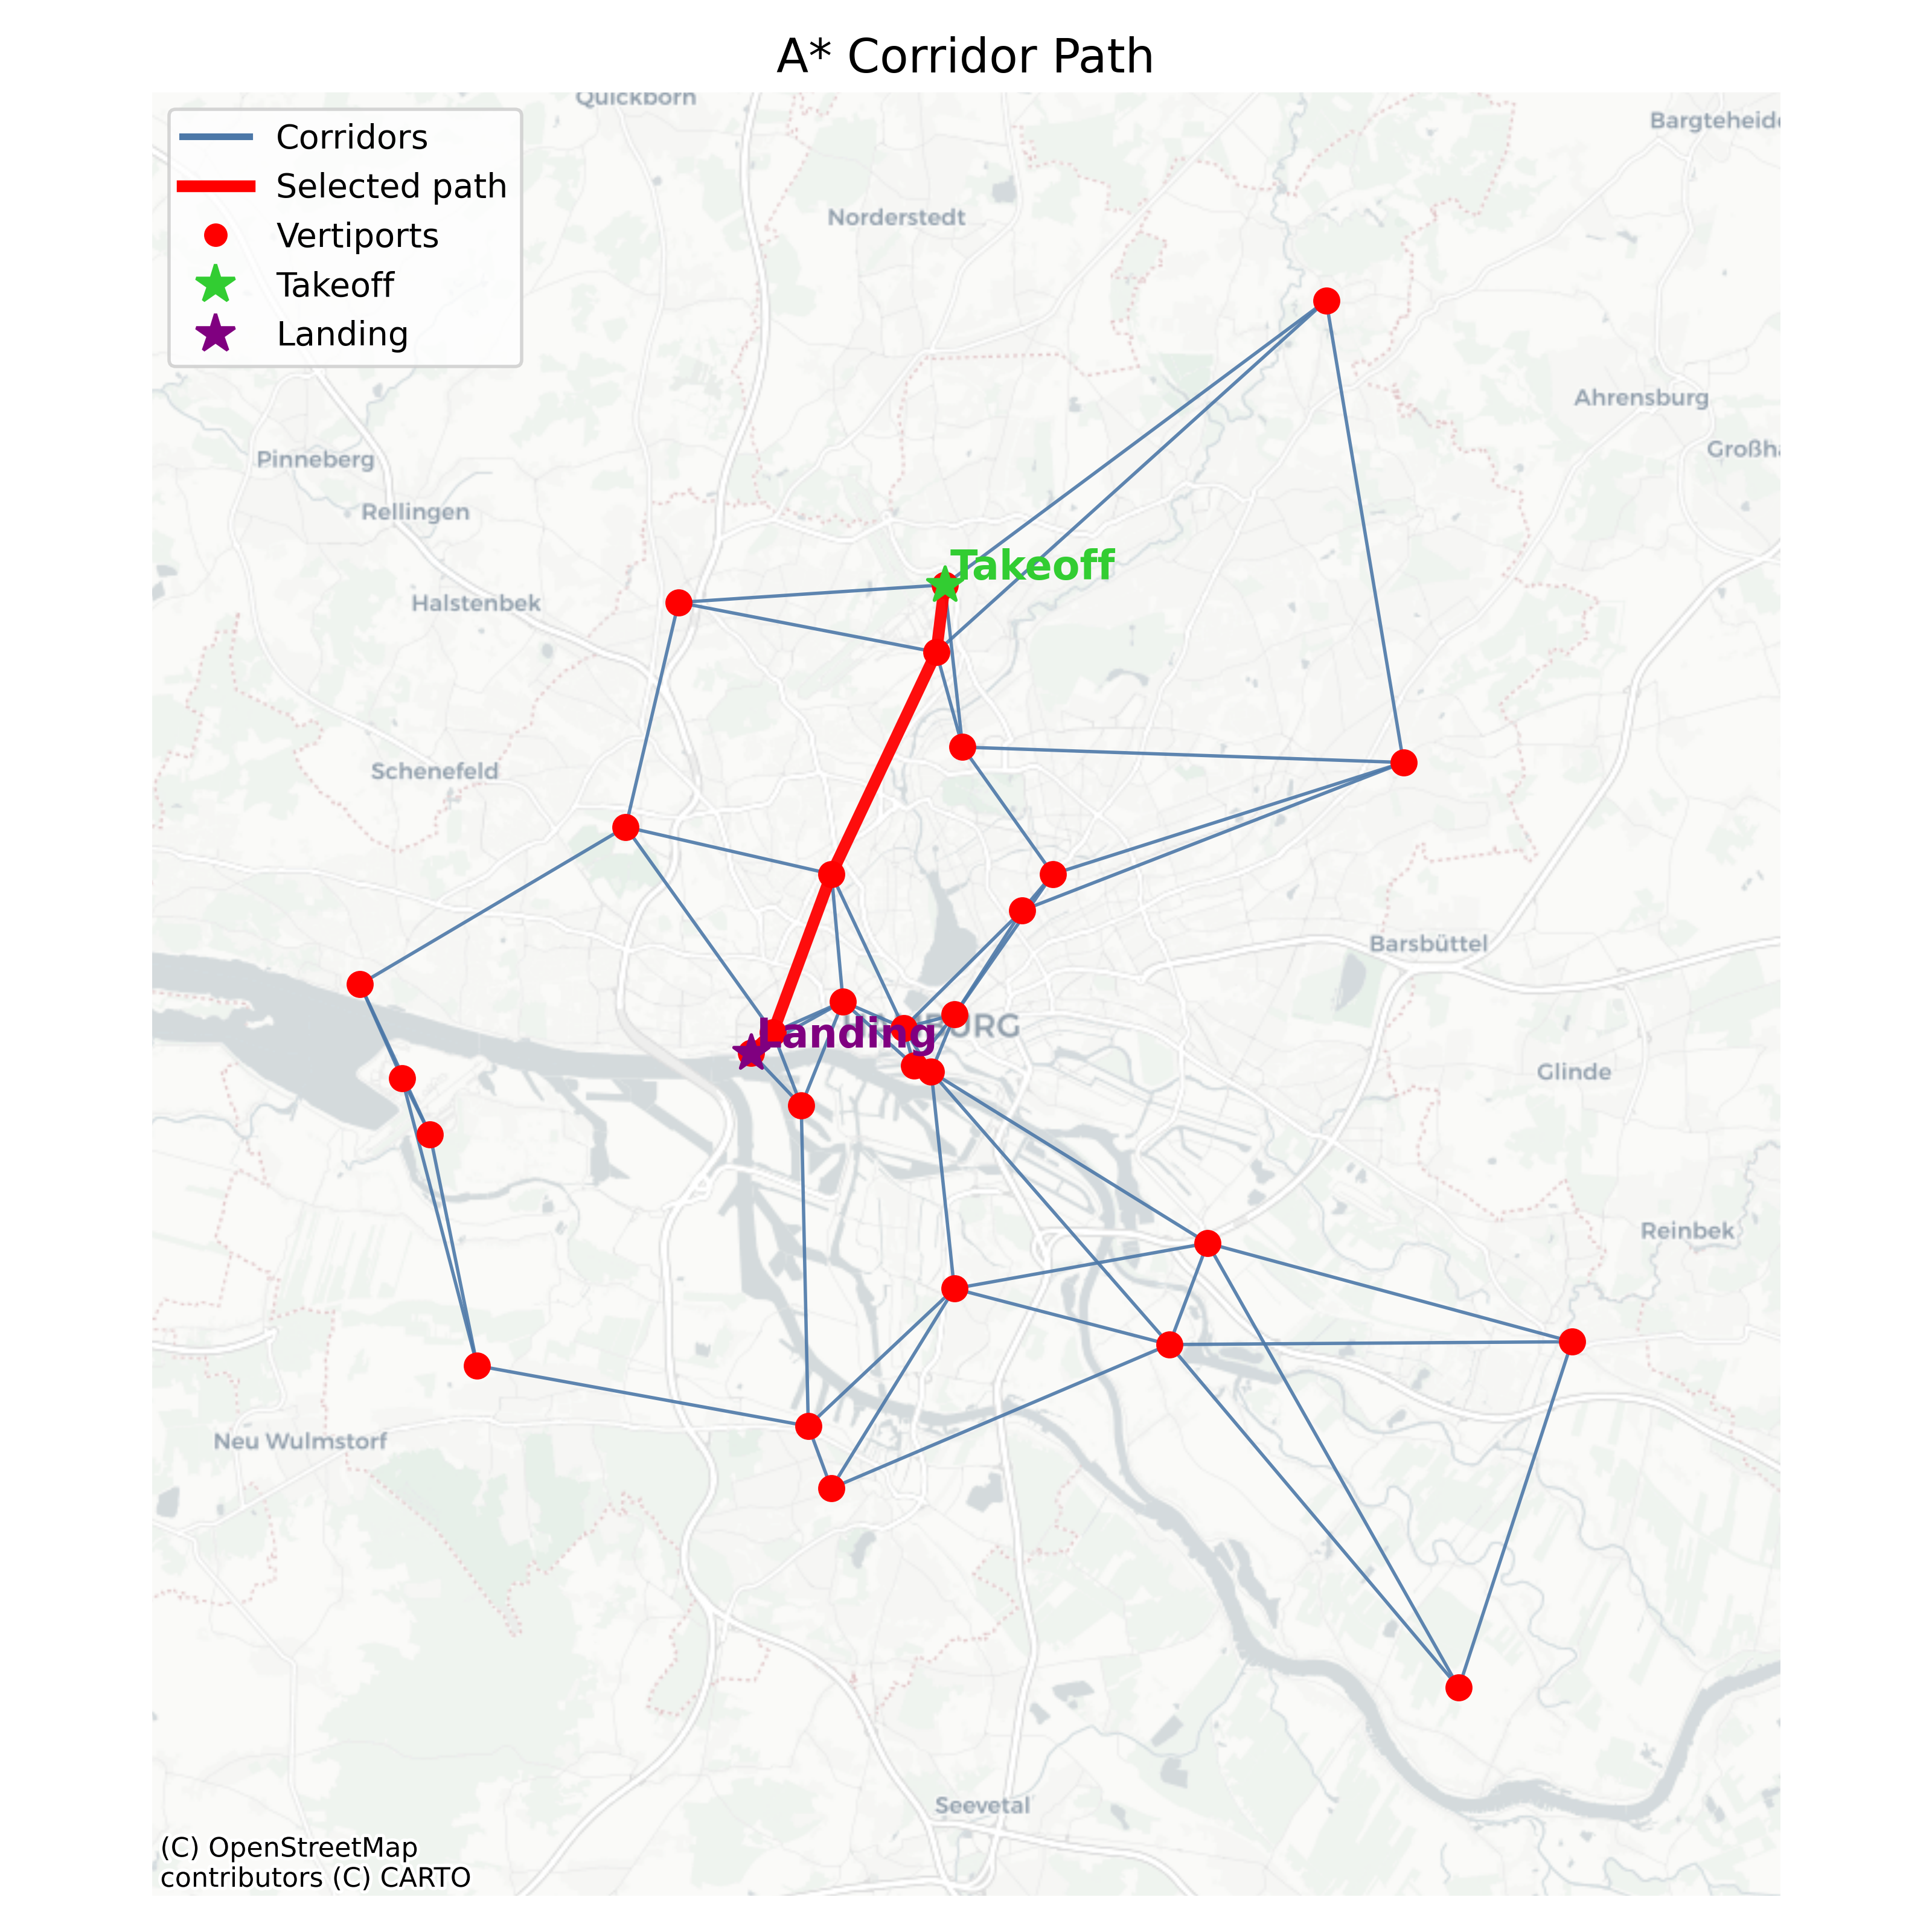
\includegraphics[width=0.5\textwidth]{results/trajectoryB_map.png}
  \caption{Planned reference trajectory (Trajectory B) from \(s\) to \(d\) over the Hamburg corridor network.}
  \label{fig:trajB_map}
\end{figure}

\subsubsection*{Front-end Visualization (Cesium)}
Figure~\ref{fig:trajB_cesium} shows the planned Trajectory~B in the Cesium-based front end. 
The left panel displays the full 3D route, while the right panel zooms into 
the departure phase, illustrating the short initial leg and the early turning manoeuvre 
required to reach the first waypoint.

\begin{figure}[H]
  \centering
  \begin{subfigure}[t]{0.48\textwidth}
    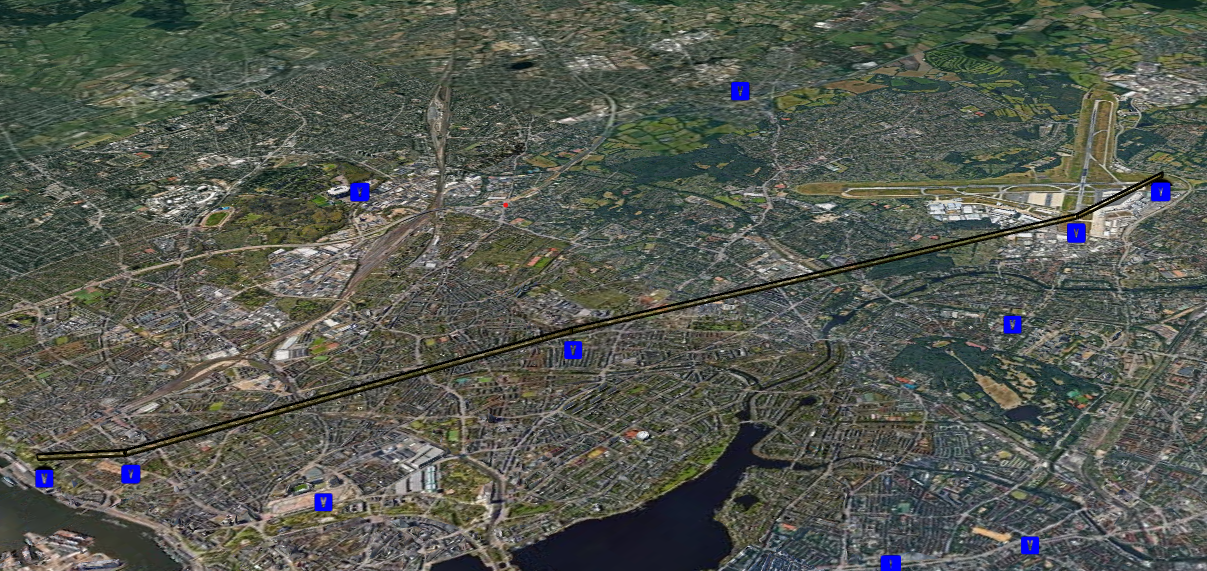
\includegraphics[width=\textwidth]{results/trajectoryB_cesium_full.png}
    \caption{Planned route (Trajectory B): full 3D corridor context.}
  \end{subfigure}
  \hfill
  \begin{subfigure}[t]{0.48\textwidth}
    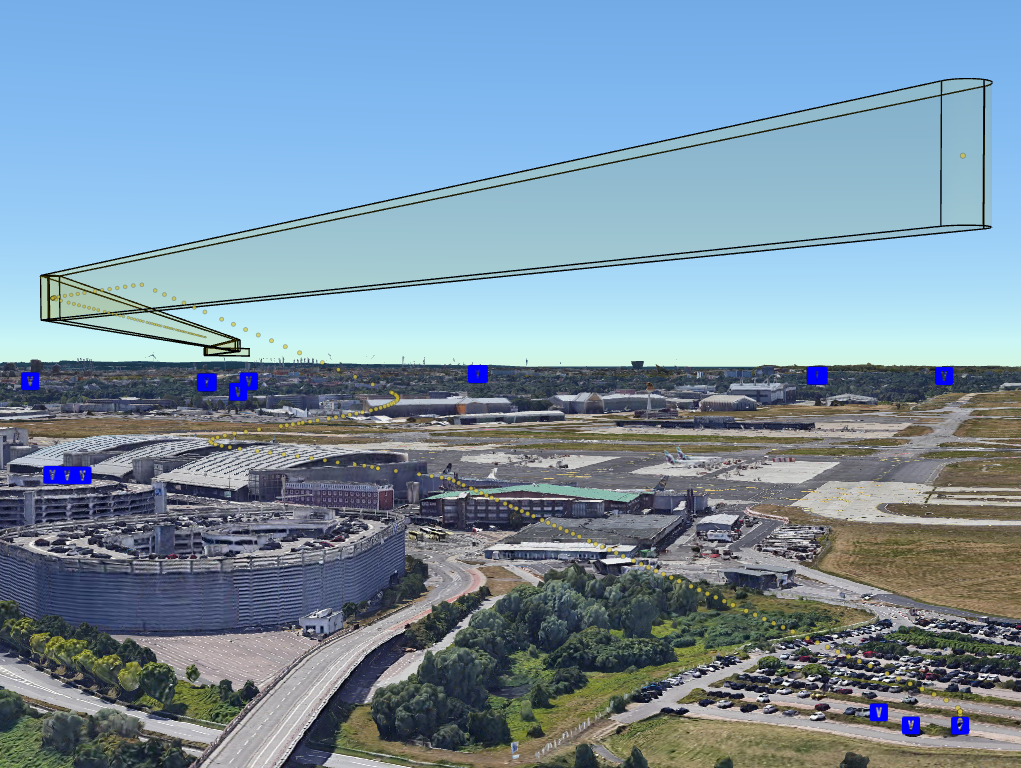
\includegraphics[width=\textwidth]{results/trajectoryB_cesium_takeoff.png}
    \caption{Planned route (Trajectory B): zoom on take-off and initial turning manoeuvre.}
  \end{subfigure}
  \caption{Cesium-based visualization of the planned Trajectory~B in the front end. Left: full route; right: take-off segment.}
  \label{fig:trajB_cesium}
\end{figure}

\subsubsection*{Kinematic Profiles}
\begin{figure}[H]
  \centering
  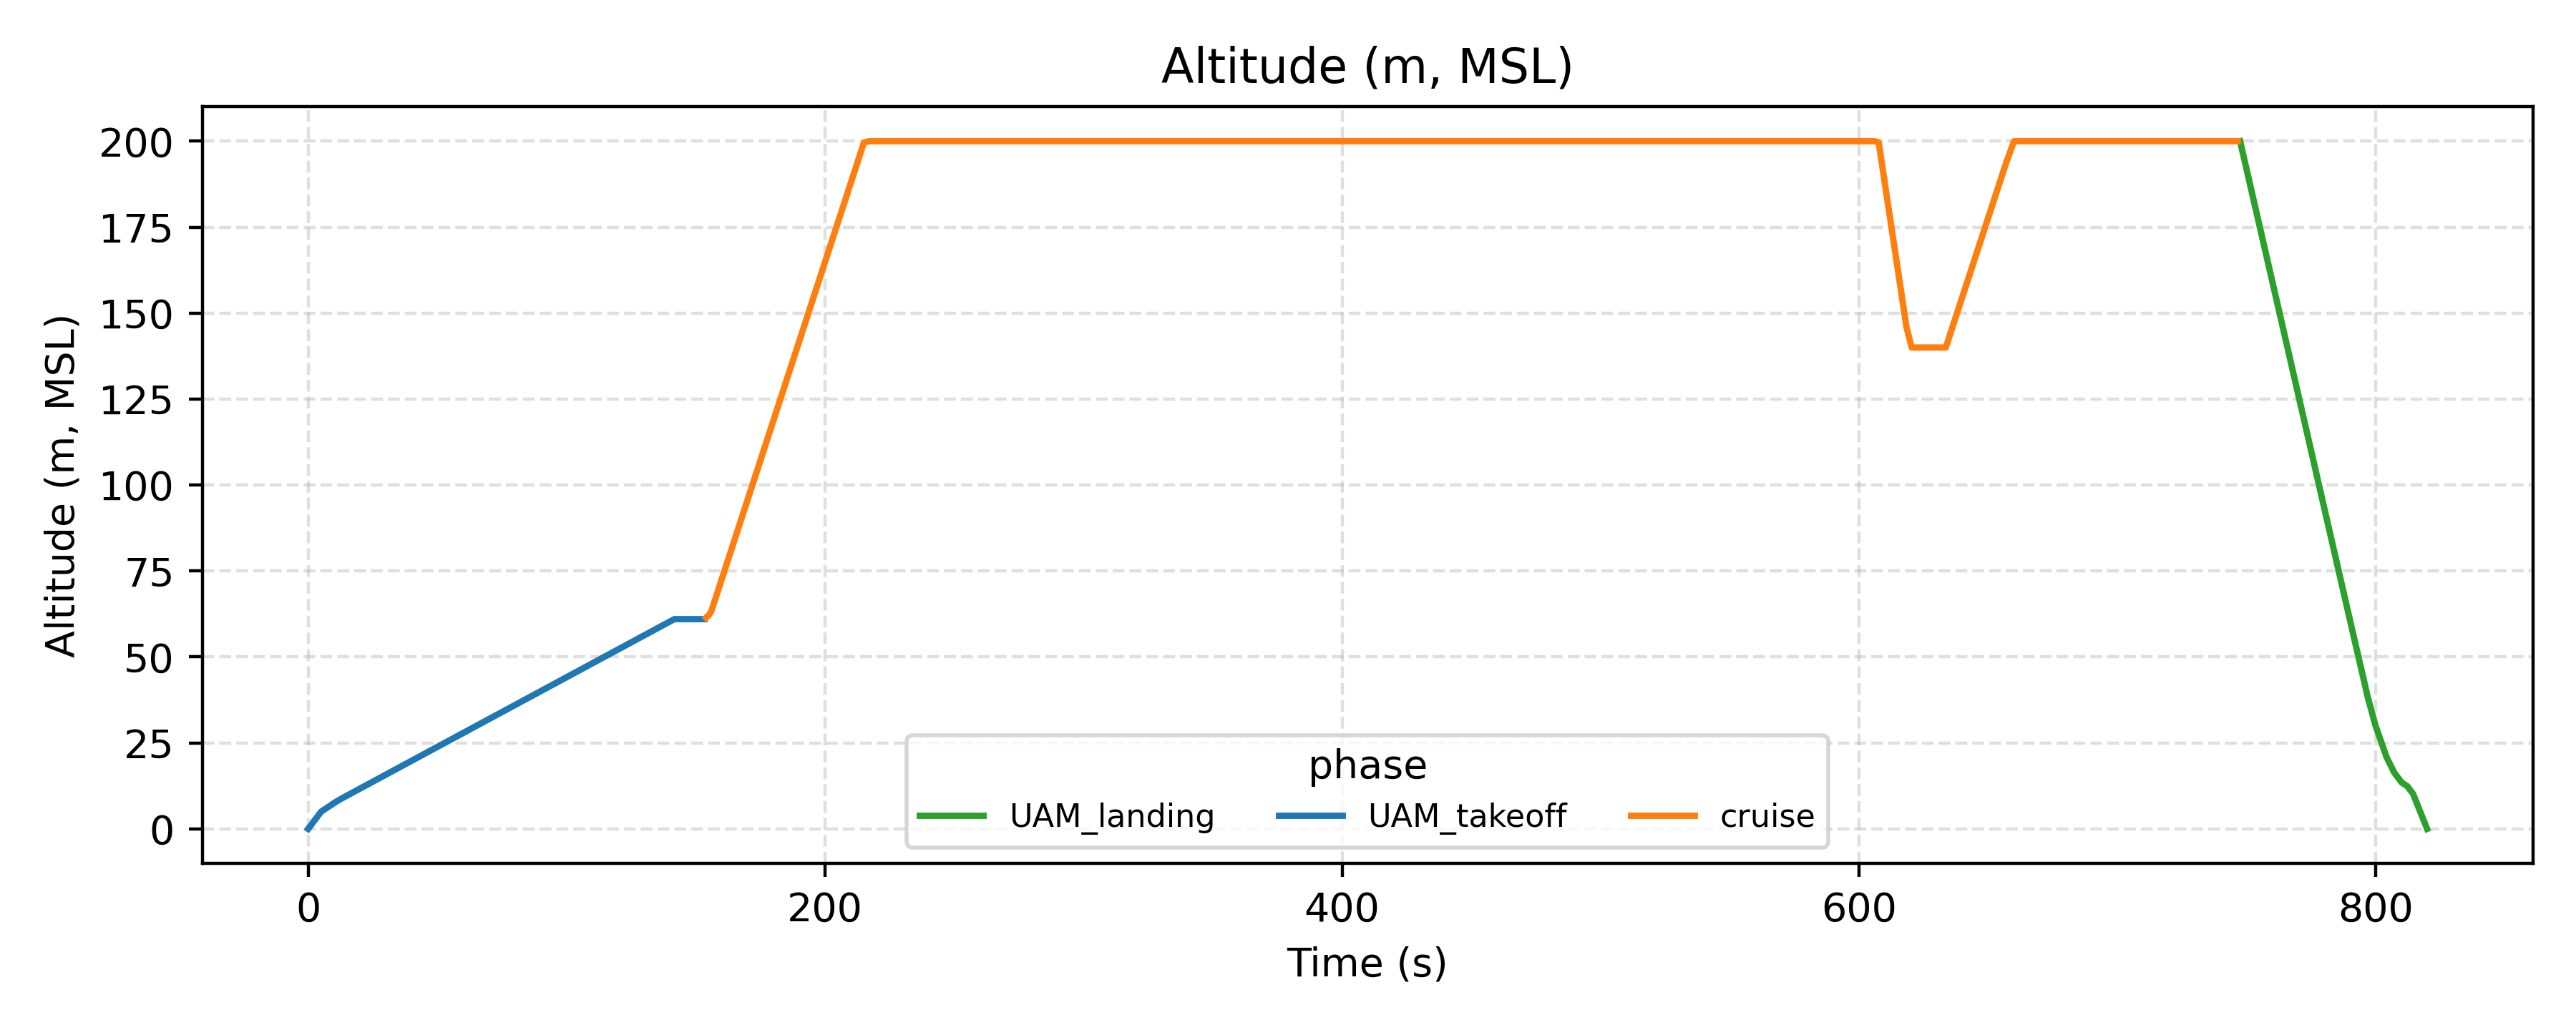
\includegraphics[width=0.86\textwidth]{results/trajectoryB_altitude.png}
  \caption{Planned altitude profile \(H(\tau)\) for Trajectory B (cruise layer near \SI{200}{m} AGL).}
  \label{fig:trajB_alt}
\end{figure}

\begin{figure}[H]
  \centering
  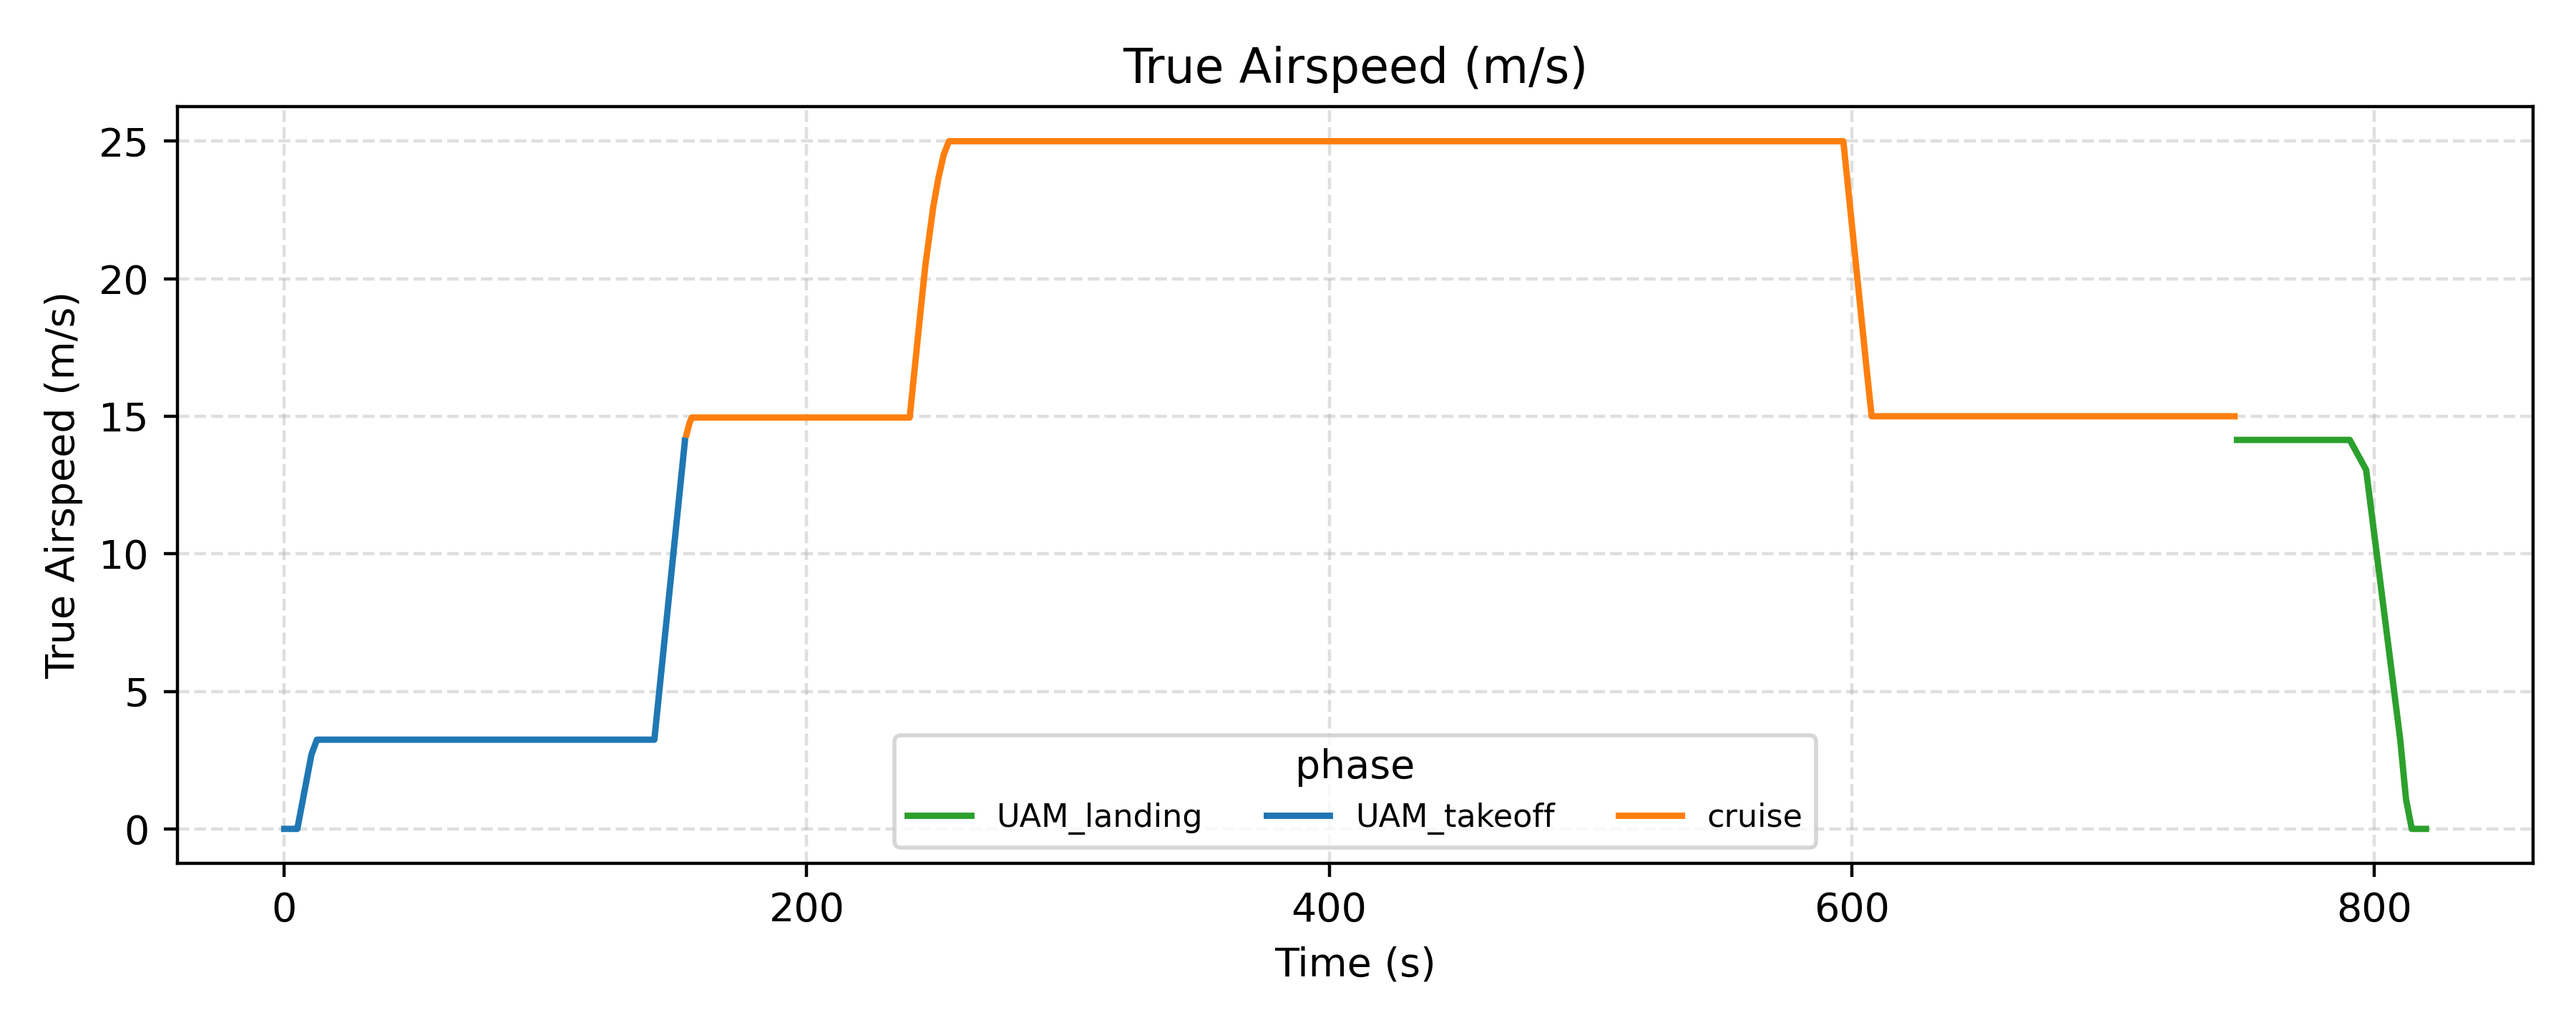
\includegraphics[width=0.86\textwidth]{results/trajectoryB_TAS.png}
  \caption{Planned true airspeed (TAS) profile for Trajectory B.}
  \label{fig:trajB_tas}
\end{figure}

\begin{figure}[H]
  \centering
  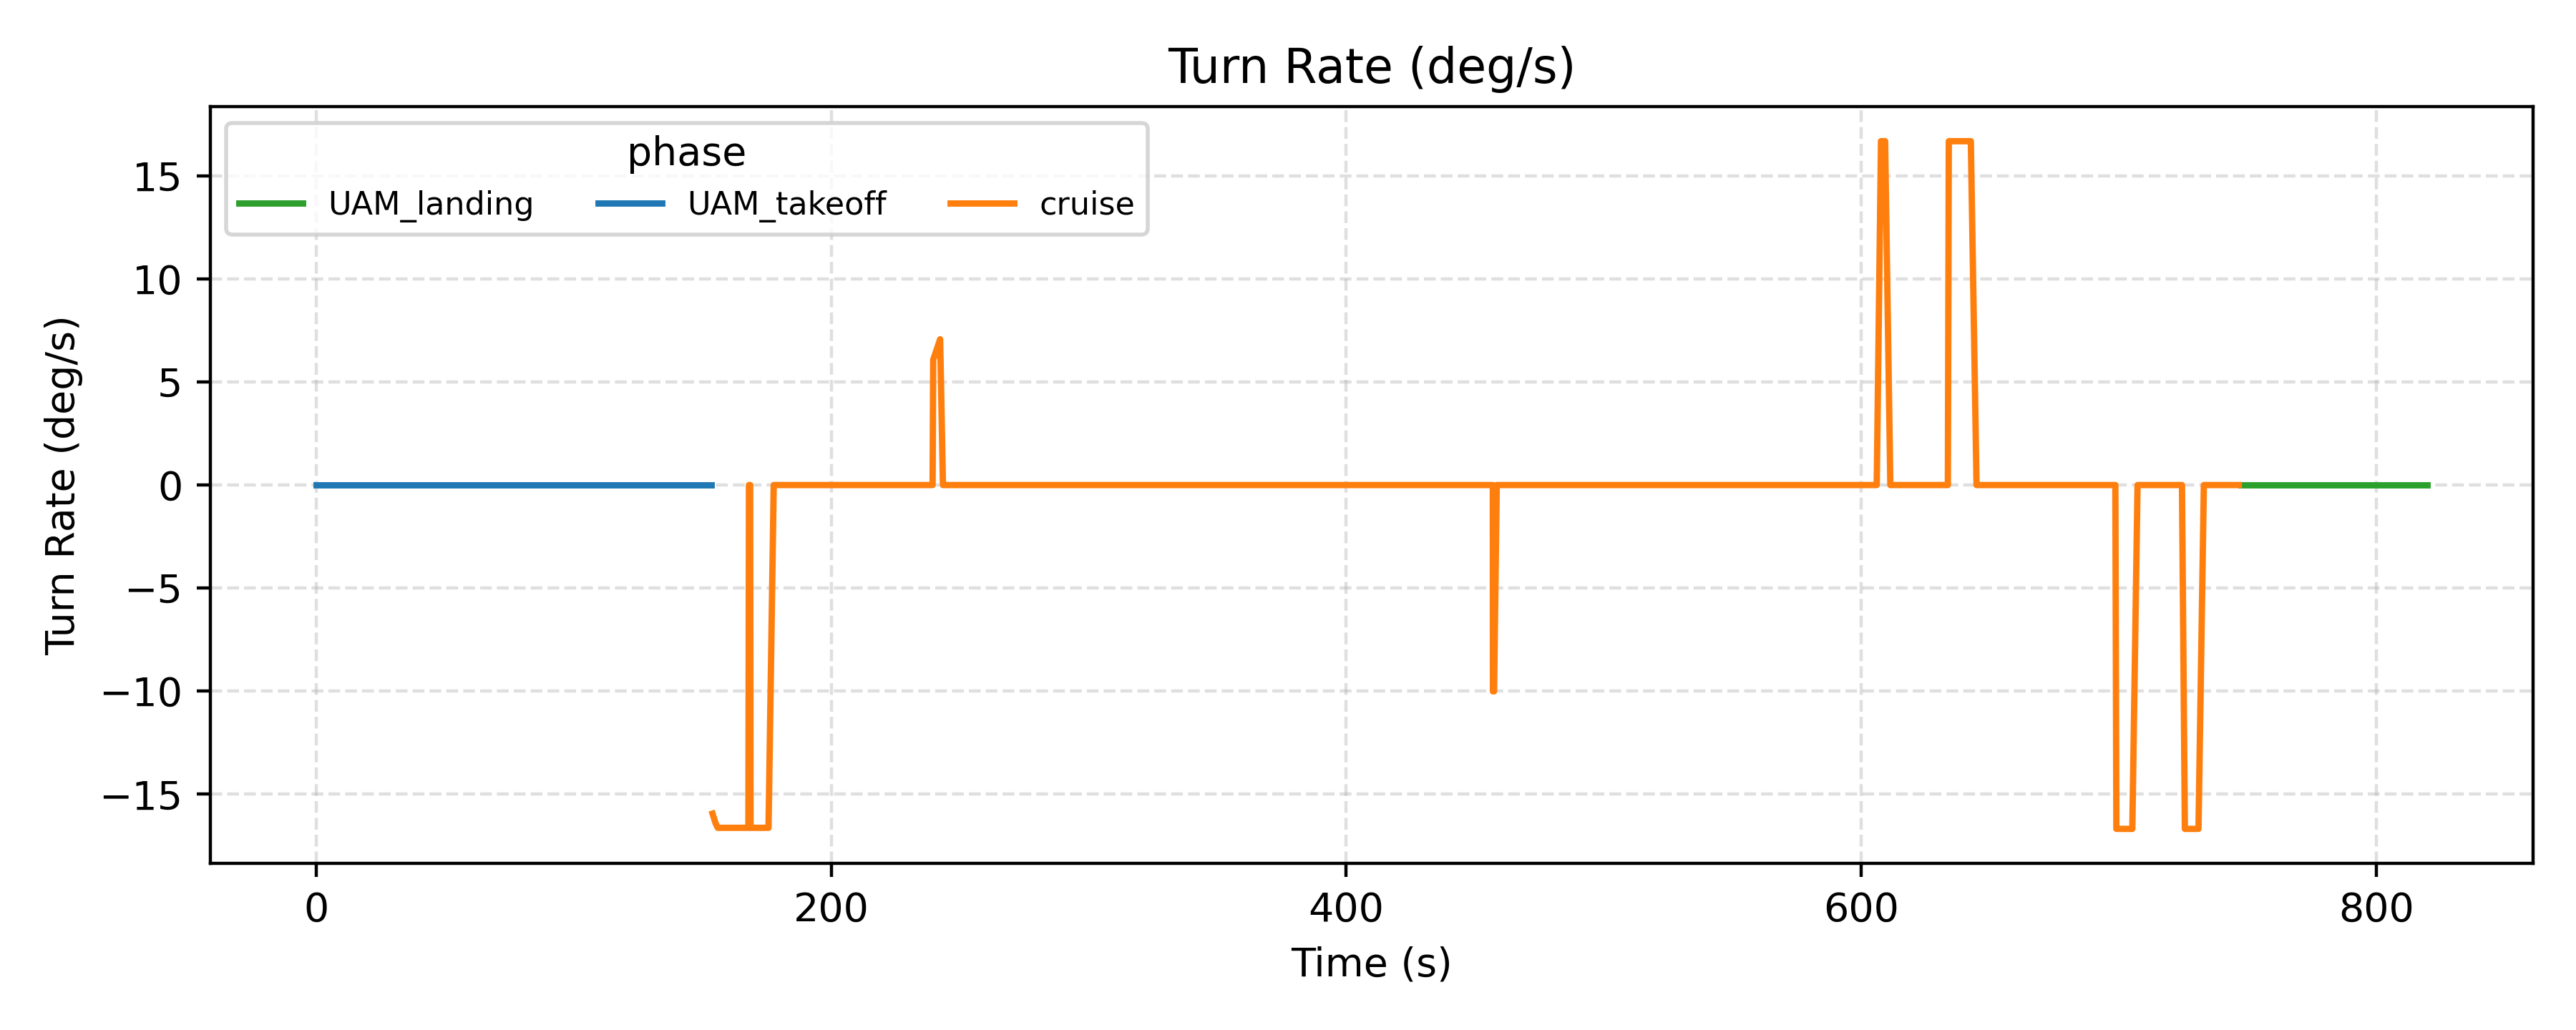
\includegraphics[width=0.86\textwidth]{results/trajectoryB_turn.png}
  \caption{Planned turn-rate profile \(\dot{\psi}(\tau)\) for Trajectory B (deg/s).}
  \label{fig:trajB_turn}
\end{figure}

\begin{figure}[H]
  \centering
  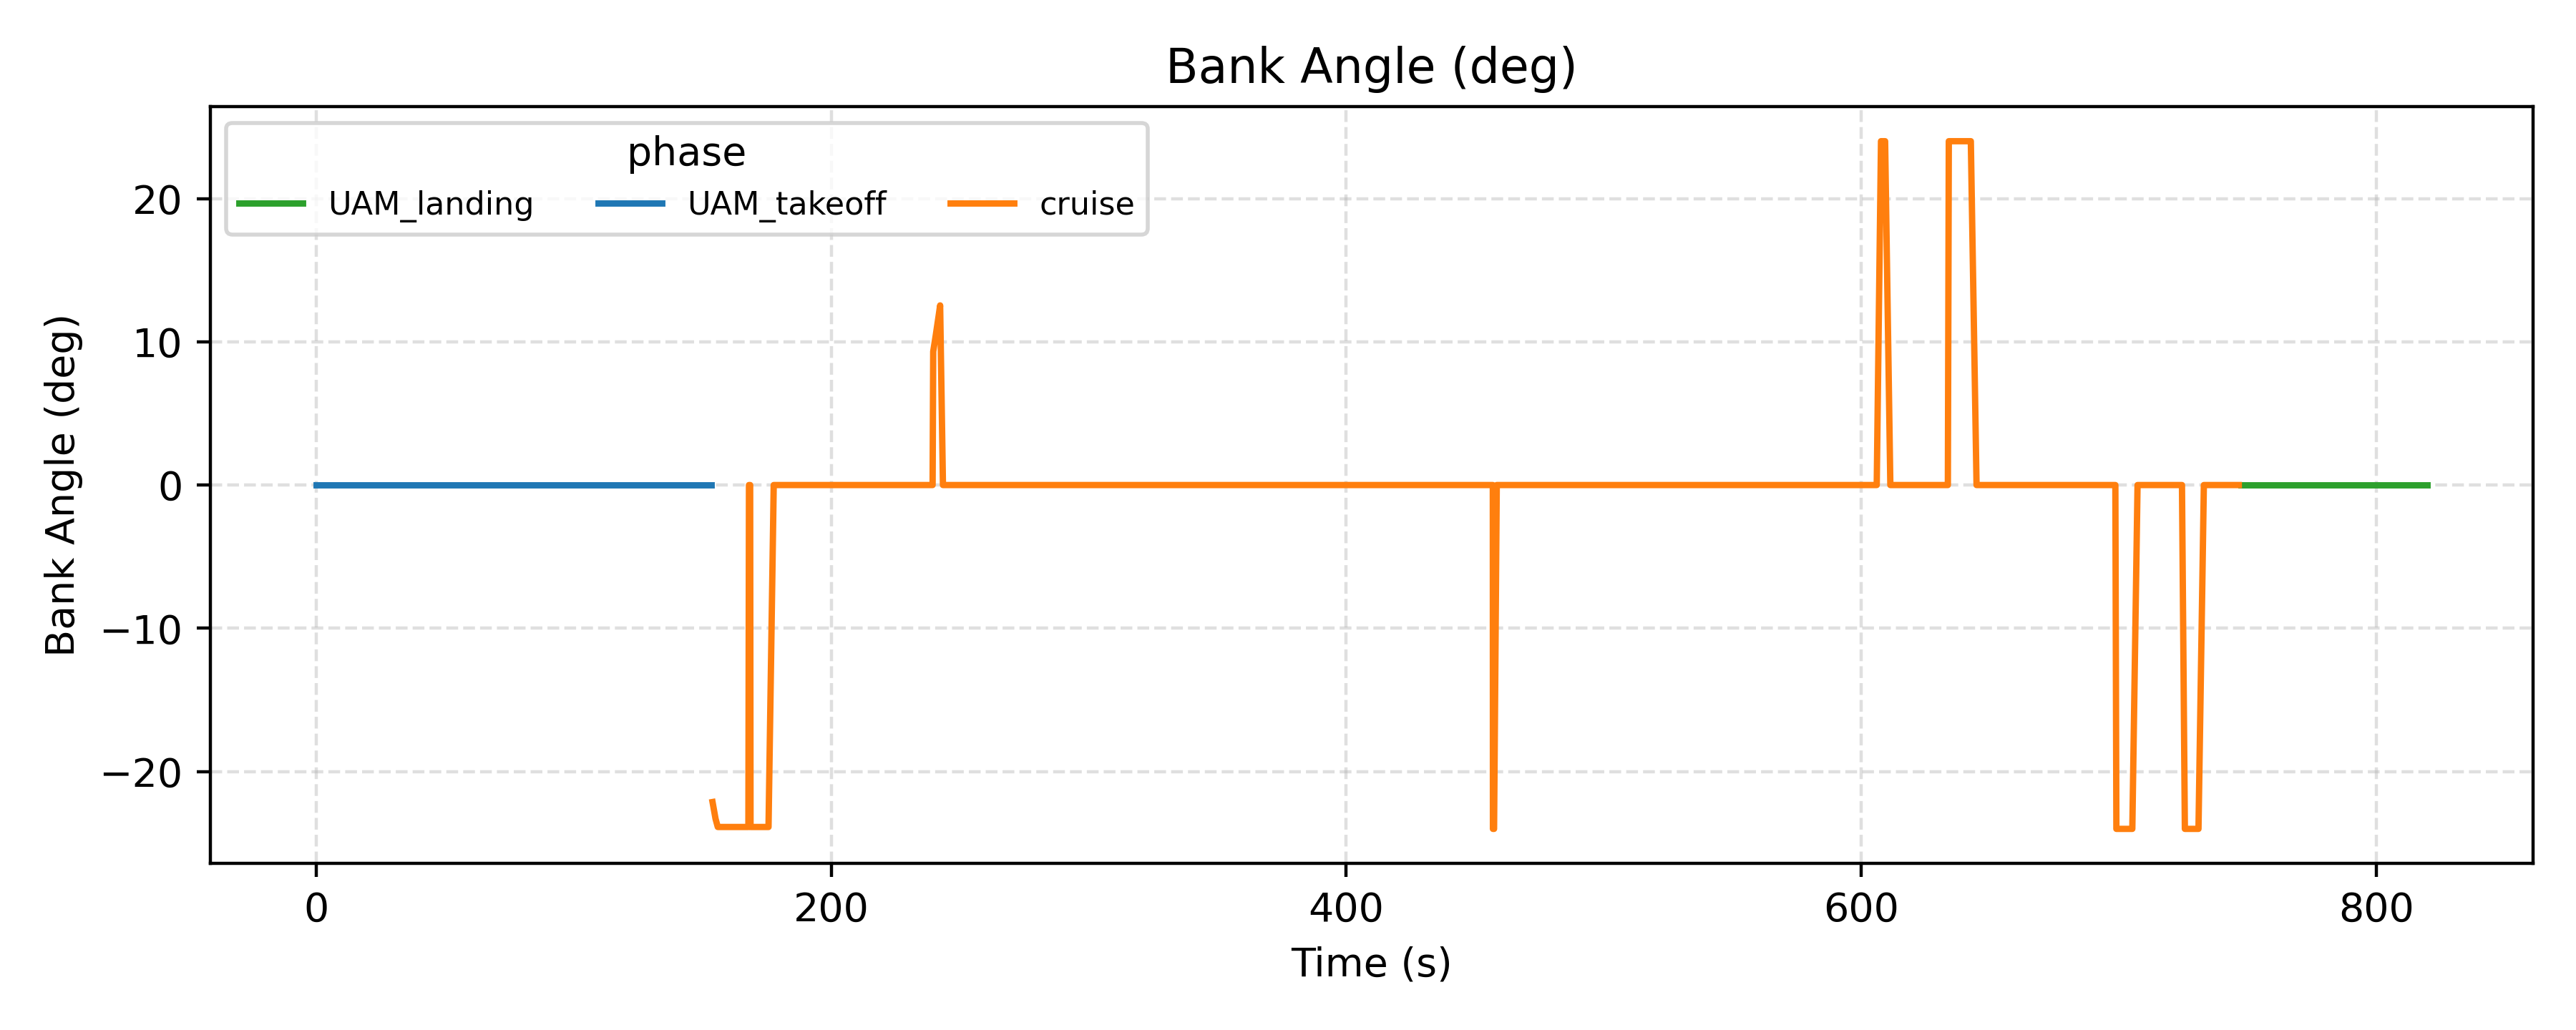
\includegraphics[width=0.86\textwidth]{results/trajectoryB_bank.png}
  \caption{Planned bank-angle profile $\phi(\tau)$ for Trajectory B (deg).}
  \label{fig:trajB_bank}
\end{figure}

\subsubsection*{Summary Statistics}
\begin{table}[H]
  \centering
  \caption{Summary statistics for the planned reference Trajectory B.}
  \label{tab:trajB_summary}
  \begin{tabular}{l r}
    \toprule
    Points & \num{500} \\
    Total time $T$ (s) & \num{819.81} \\
    Total time $T$ (min) & \num{13.66} \\
    Total distance $L$ (km) & \num{13.79} \\
    Mean TAS (m/s) & \num{16.67} \\
    Peak bank angle $\max \phi$ (deg) & \num{24.01} \\
    Peak turn rate $\max \dot{\psi}$ (deg/s) & \num{16.68} \\
    Peak climb rate $\max \dot{H}$ (m/s) & \num{6.63} \\
    \bottomrule
  \end{tabular}
\end{table}

\section{Conflict Handling}
\label{sec:results_conflicts}

In this section, the ability of the framework to detect and resolve conflicts is demonstrated.
Two representative trajectories were selected within the Hamburg corridor network
(trajectory \texttt{HAM~$\rightarrow$~WILH} and trajectory \texttt{TTNB~$\rightarrow$~HOHE}),
whose initially planned routes overlap spatially and temporally. This setup provides
a suitable test case for illustrating both the detection of a conflict and its
subsequent resolution through lateral re-routing.

\subsection{Conflict Detection}
The candidate routes were submitted to the NDMap conflict detection module
(Sec.~\ref{sec:ndmap}), which evaluates trajectory pairs in four-dimensional space
(longitude, latitude, altitude, time).  
Figure~\ref{fig:conflict_initial} shows the initially planned routes,
with the overlapping edge segment highlighted in red.  
NDMap reported a conflict interval
\([\tau_{\text{start}}, \tau_{\text{end}}] = [654.2\,\text{s}, 664.8\,\text{s}]\),
indicating that both UAM trajectories would occupy the same corridor segment
within a temporal overlap of approximately \SI{10.6}{s}.

\begin{figure}[H]
  \centering
  \begin{subfigure}[t]{0.48\textwidth}
    \centering
    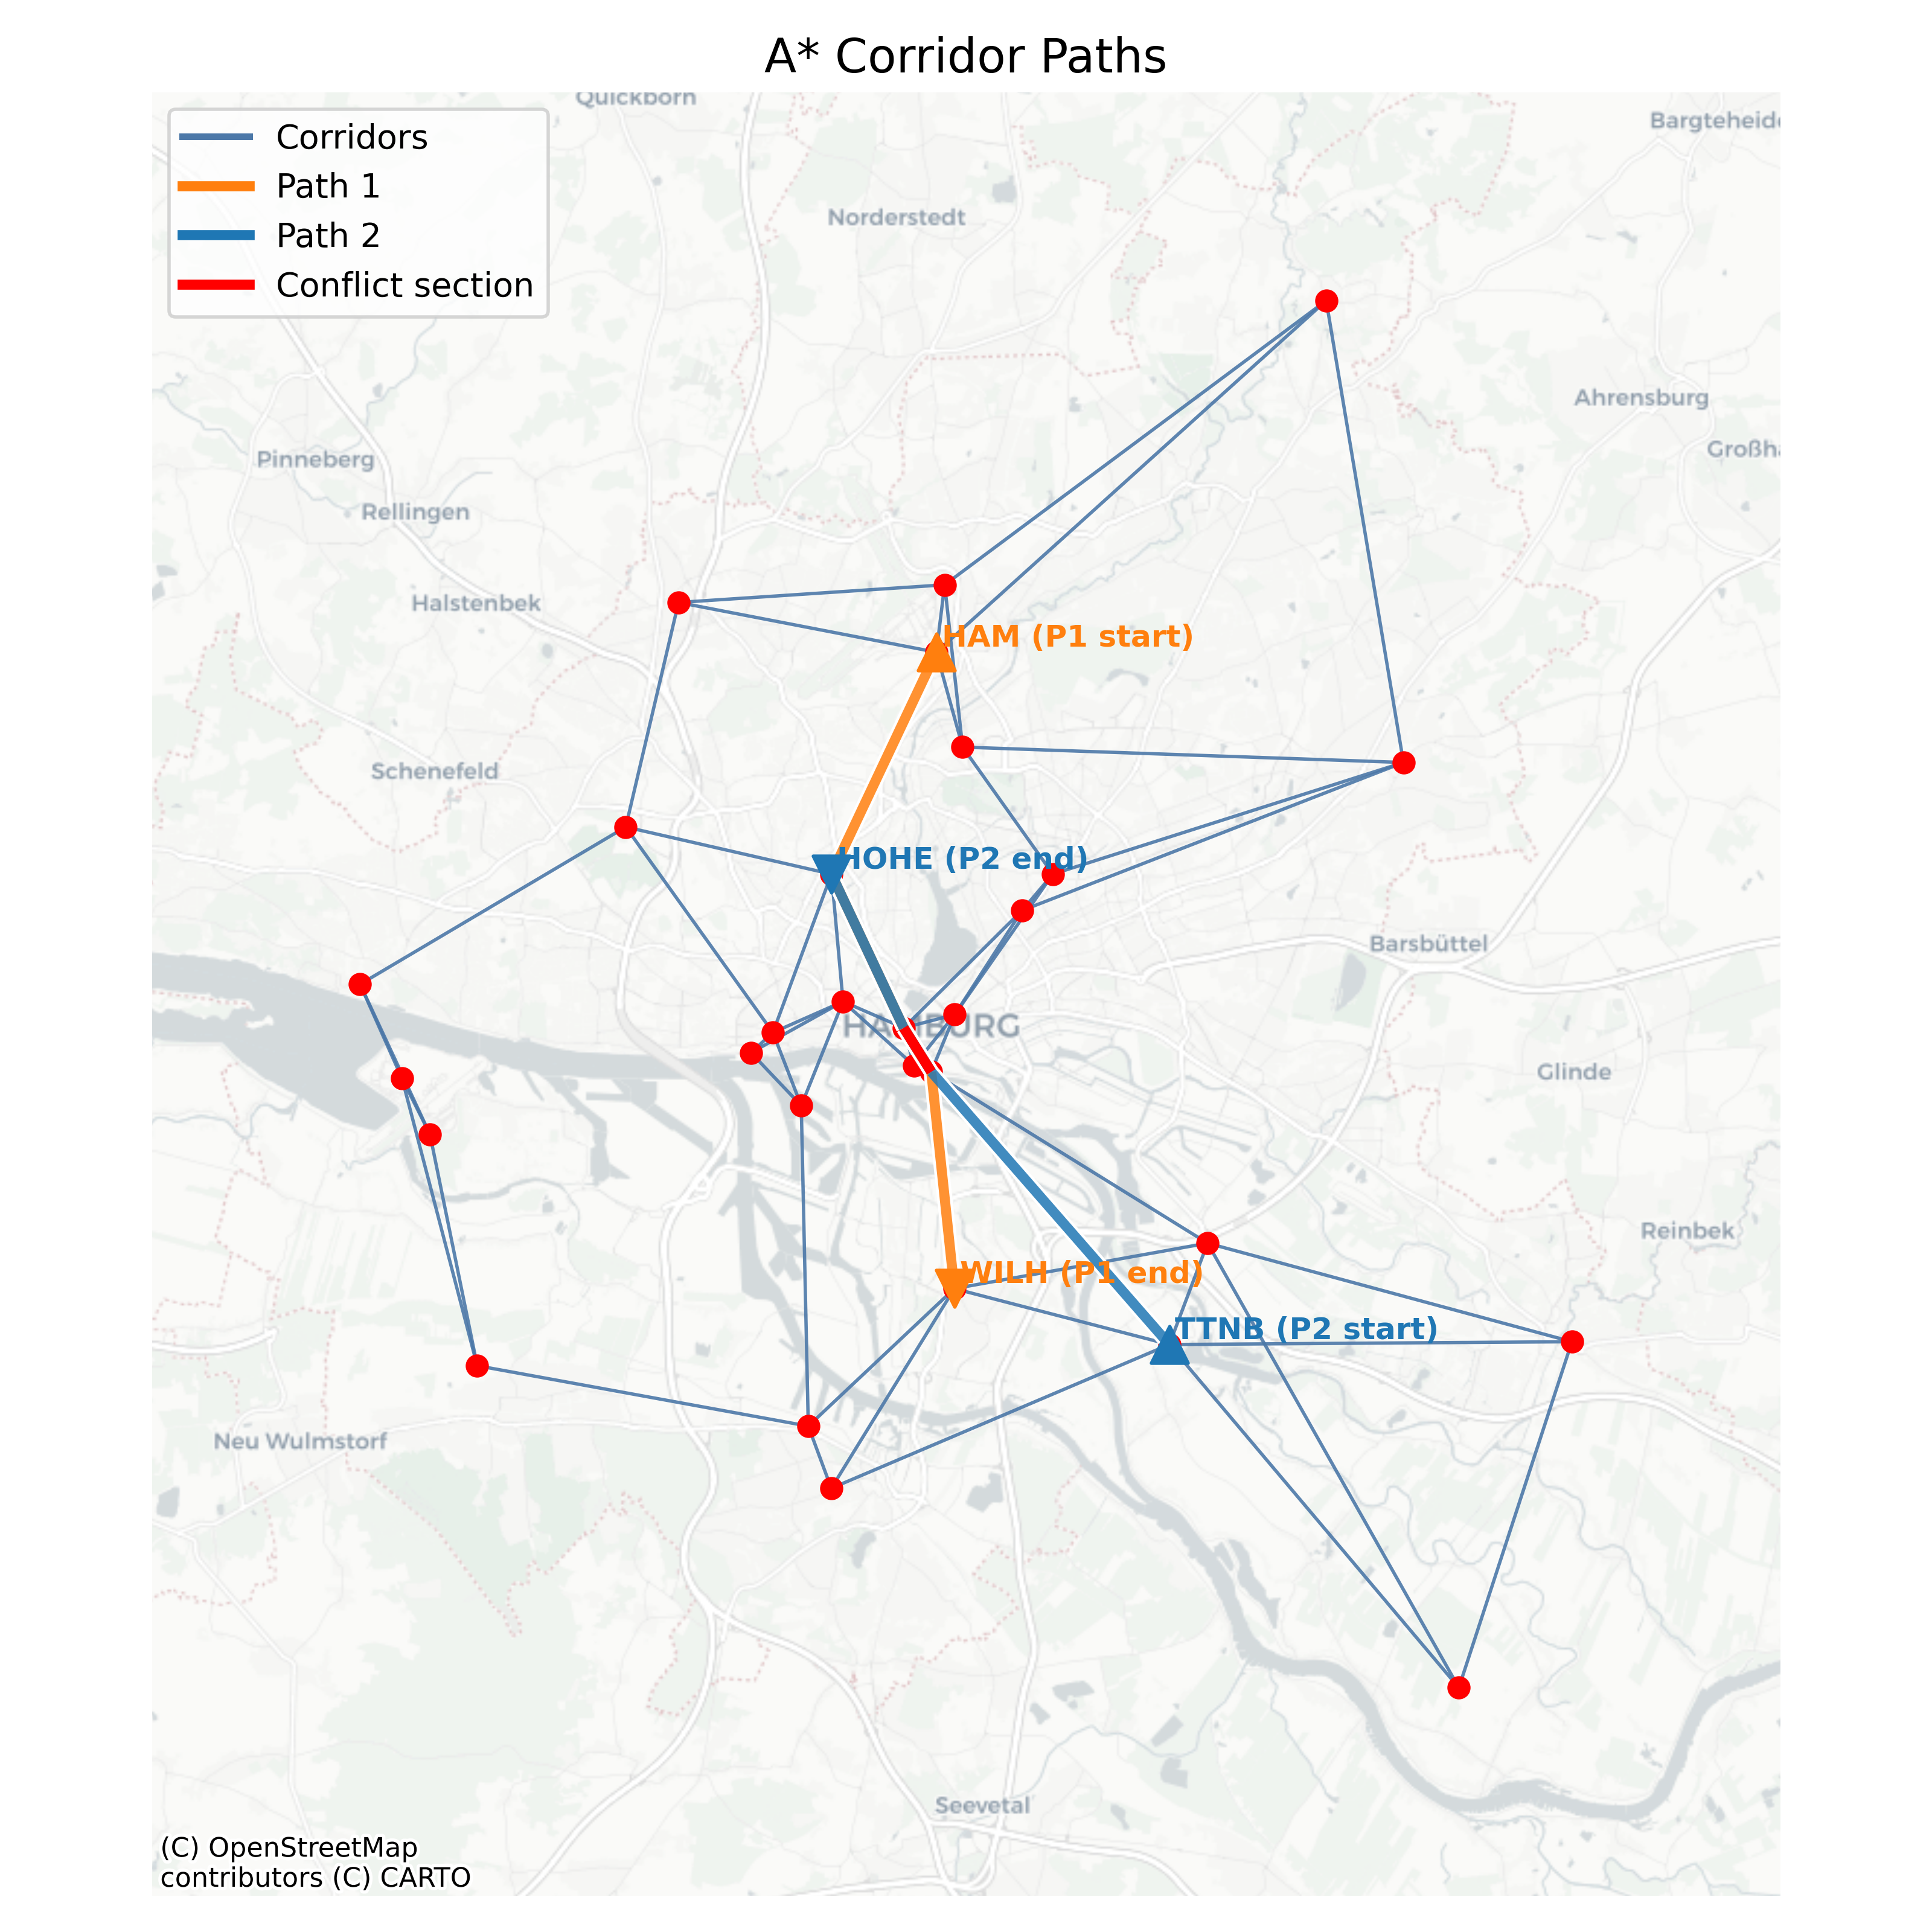
\includegraphics[width=\textwidth]{results/corridors_multiple_paths.png}
    \caption{Initial planned routes for \texttt{HAM~$\rightarrow$~WILH} and \texttt{TTNB~$\rightarrow$~HOHE}; the overlapping planned corridor segment (conflict) is marked in red.}
    \label{fig:conflict_initial}
  \end{subfigure}
  \hfill
  \begin{subfigure}[t]{0.48\textwidth}
    \centering
    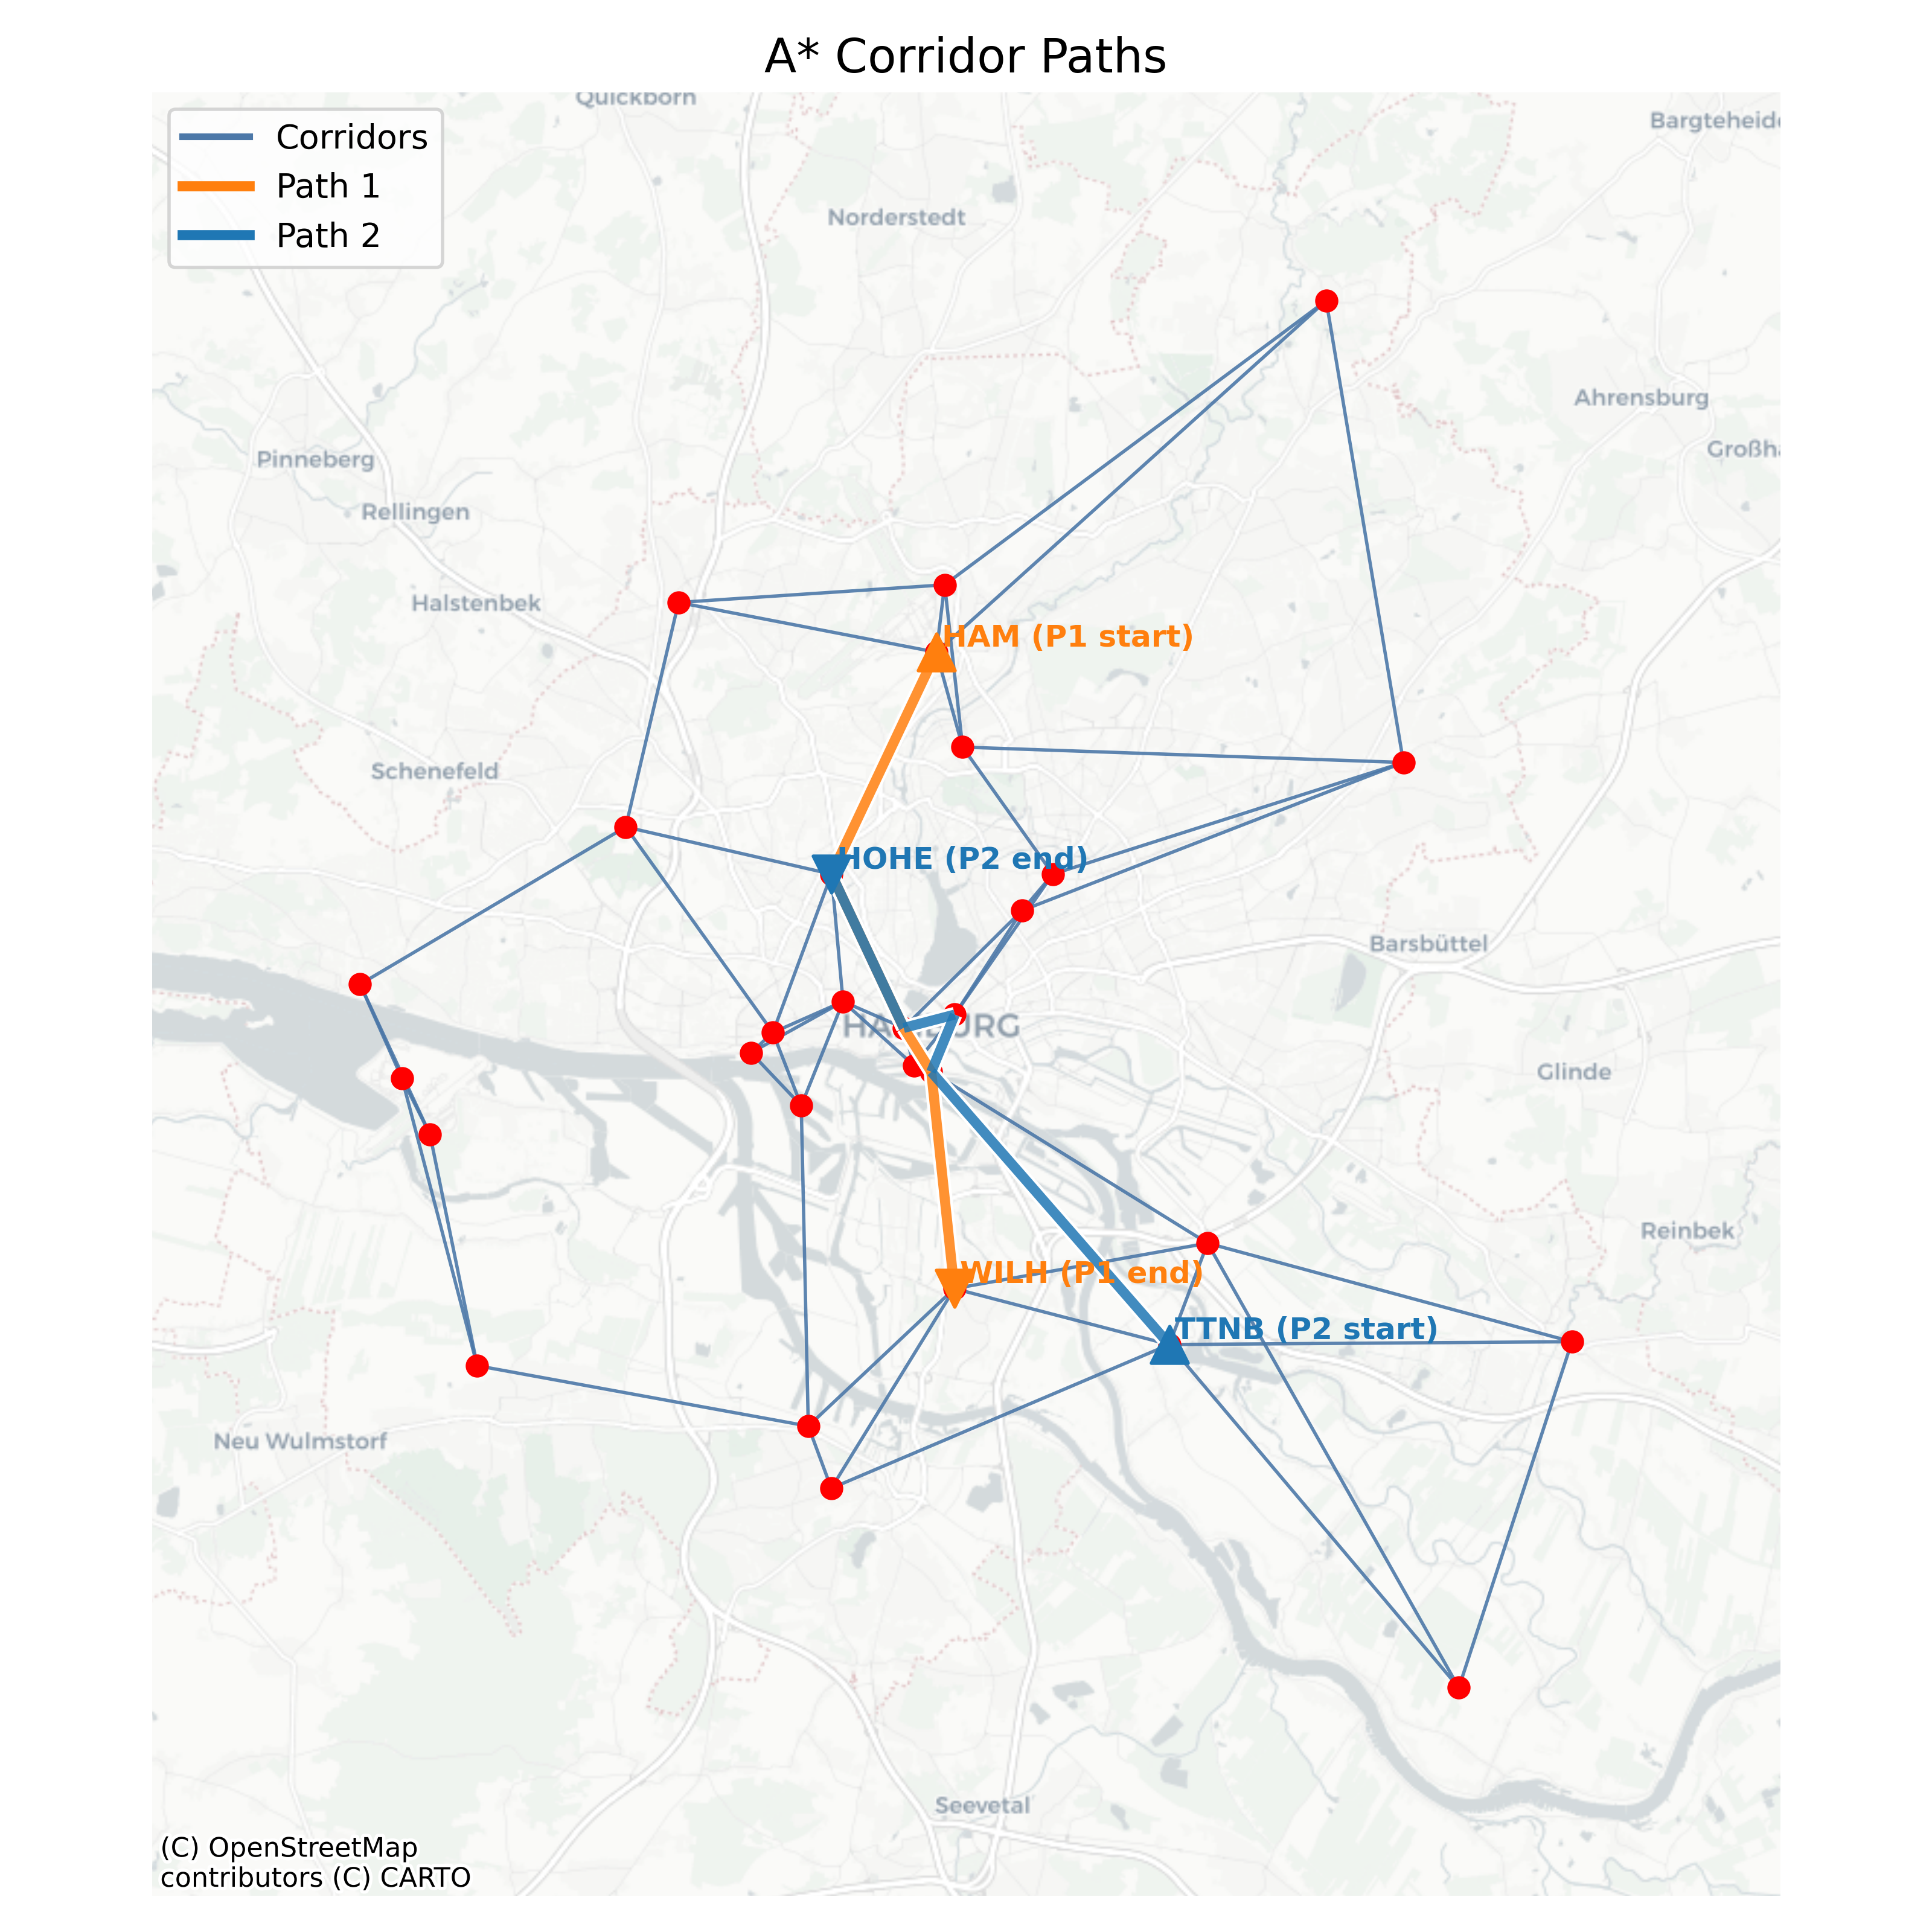
\includegraphics[width=\textwidth]{results/corridors_multiple_paths_resolved.png}
    \caption{Re-planned conflict-free route for \texttt{TTNB~$\rightarrow$~HOHE}; the revised planned path avoids the previously conflicting corridor.}
    \label{fig:conflict_resolved}
  \end{subfigure}
  \caption{Comparison of conflict detection and resolution using NDMap and rerouting on planned routes.}
  \label{fig:conflict_comparison}
\end{figure}

\subsection{Conflict Resolution}
To resolve the detected conflict, the integrated rerouting strategy within the path
planning framework (Sec.~\ref{sec:astar_global}) was applied.  
Edges involved in the conflict were temporarily penalized by assigning
infinite cost in the corridor graph, effectively discouraging their selection
in subsequent planning iterations. A new A* search was then performed
for the affected trajectory (\texttt{TTNB~$\rightarrow$~HOHE}), yielding
a longer but conflict-free path.  
The outcome is shown in Fig.~\ref{fig:conflict_resolved}, where the rerouted
trajectory bypasses the overlapping corridor segment, thereby eliminating
the temporal and spatial conflict.

\subsection*{Summary}
This case study demonstrates the integrated conflict handling approach of the framework:
conflicts are detected via NDMap (Sec.~\ref{sec:ndmap}), and if present,
the route is adaptively recomputed by modifying corridor edge weights and re-running
A* search (Sec.~\ref{sec:astar_global}).  
Although this may increase the total distance and travel time, the resulting trajectory
is conflict-free, supporting safe and scalable multi-UAM operations within the Hamburg
scenario.

\subsection{Conflict Handling with Interchanged Endpoints}
A second case study considers two trajectories with interchanged start and end
vertiports: trajectory \texttt{HARB~$\rightarrow$~TTNB} and
trajectory \texttt{TTNB~$\rightarrow$~HARB}.  
In the initial planning stage, both trajectories select the same shortest route,
leading to a complete overlap of the corridor segment between the two vertiports.  
This results in an unavoidable spatial and temporal conflict when both plans are
submitted simultaneously.

\subsubsection*{Conflict Detection and Resolution}
Figure~\ref{fig:conflict_interchanged} compares the initial conflicting routes
(left) with the resolved case (right). NDMap (Sec.~\ref{sec:ndmap}) flagged the
overlapping corridor segment (red) as a conflict, with simultaneous occupancy
intervals for both trajectories.  
To resolve this, the integrated rerouting strategy (Sec.~\ref{sec:astar_global})
was applied: the conflicting edge was penalized by assigning it infinite cost,
and a new A* search was run for the later-submitted trajectory
(\texttt{TTNB~$\rightarrow$~HARB}).  
The new solution yields the second-shortest path in the network, which avoids
the overlapping corridor and ensures conflict-free operation.

\begin{figure}[H]
  \centering
  \begin{subfigure}[t]{0.48\textwidth}
    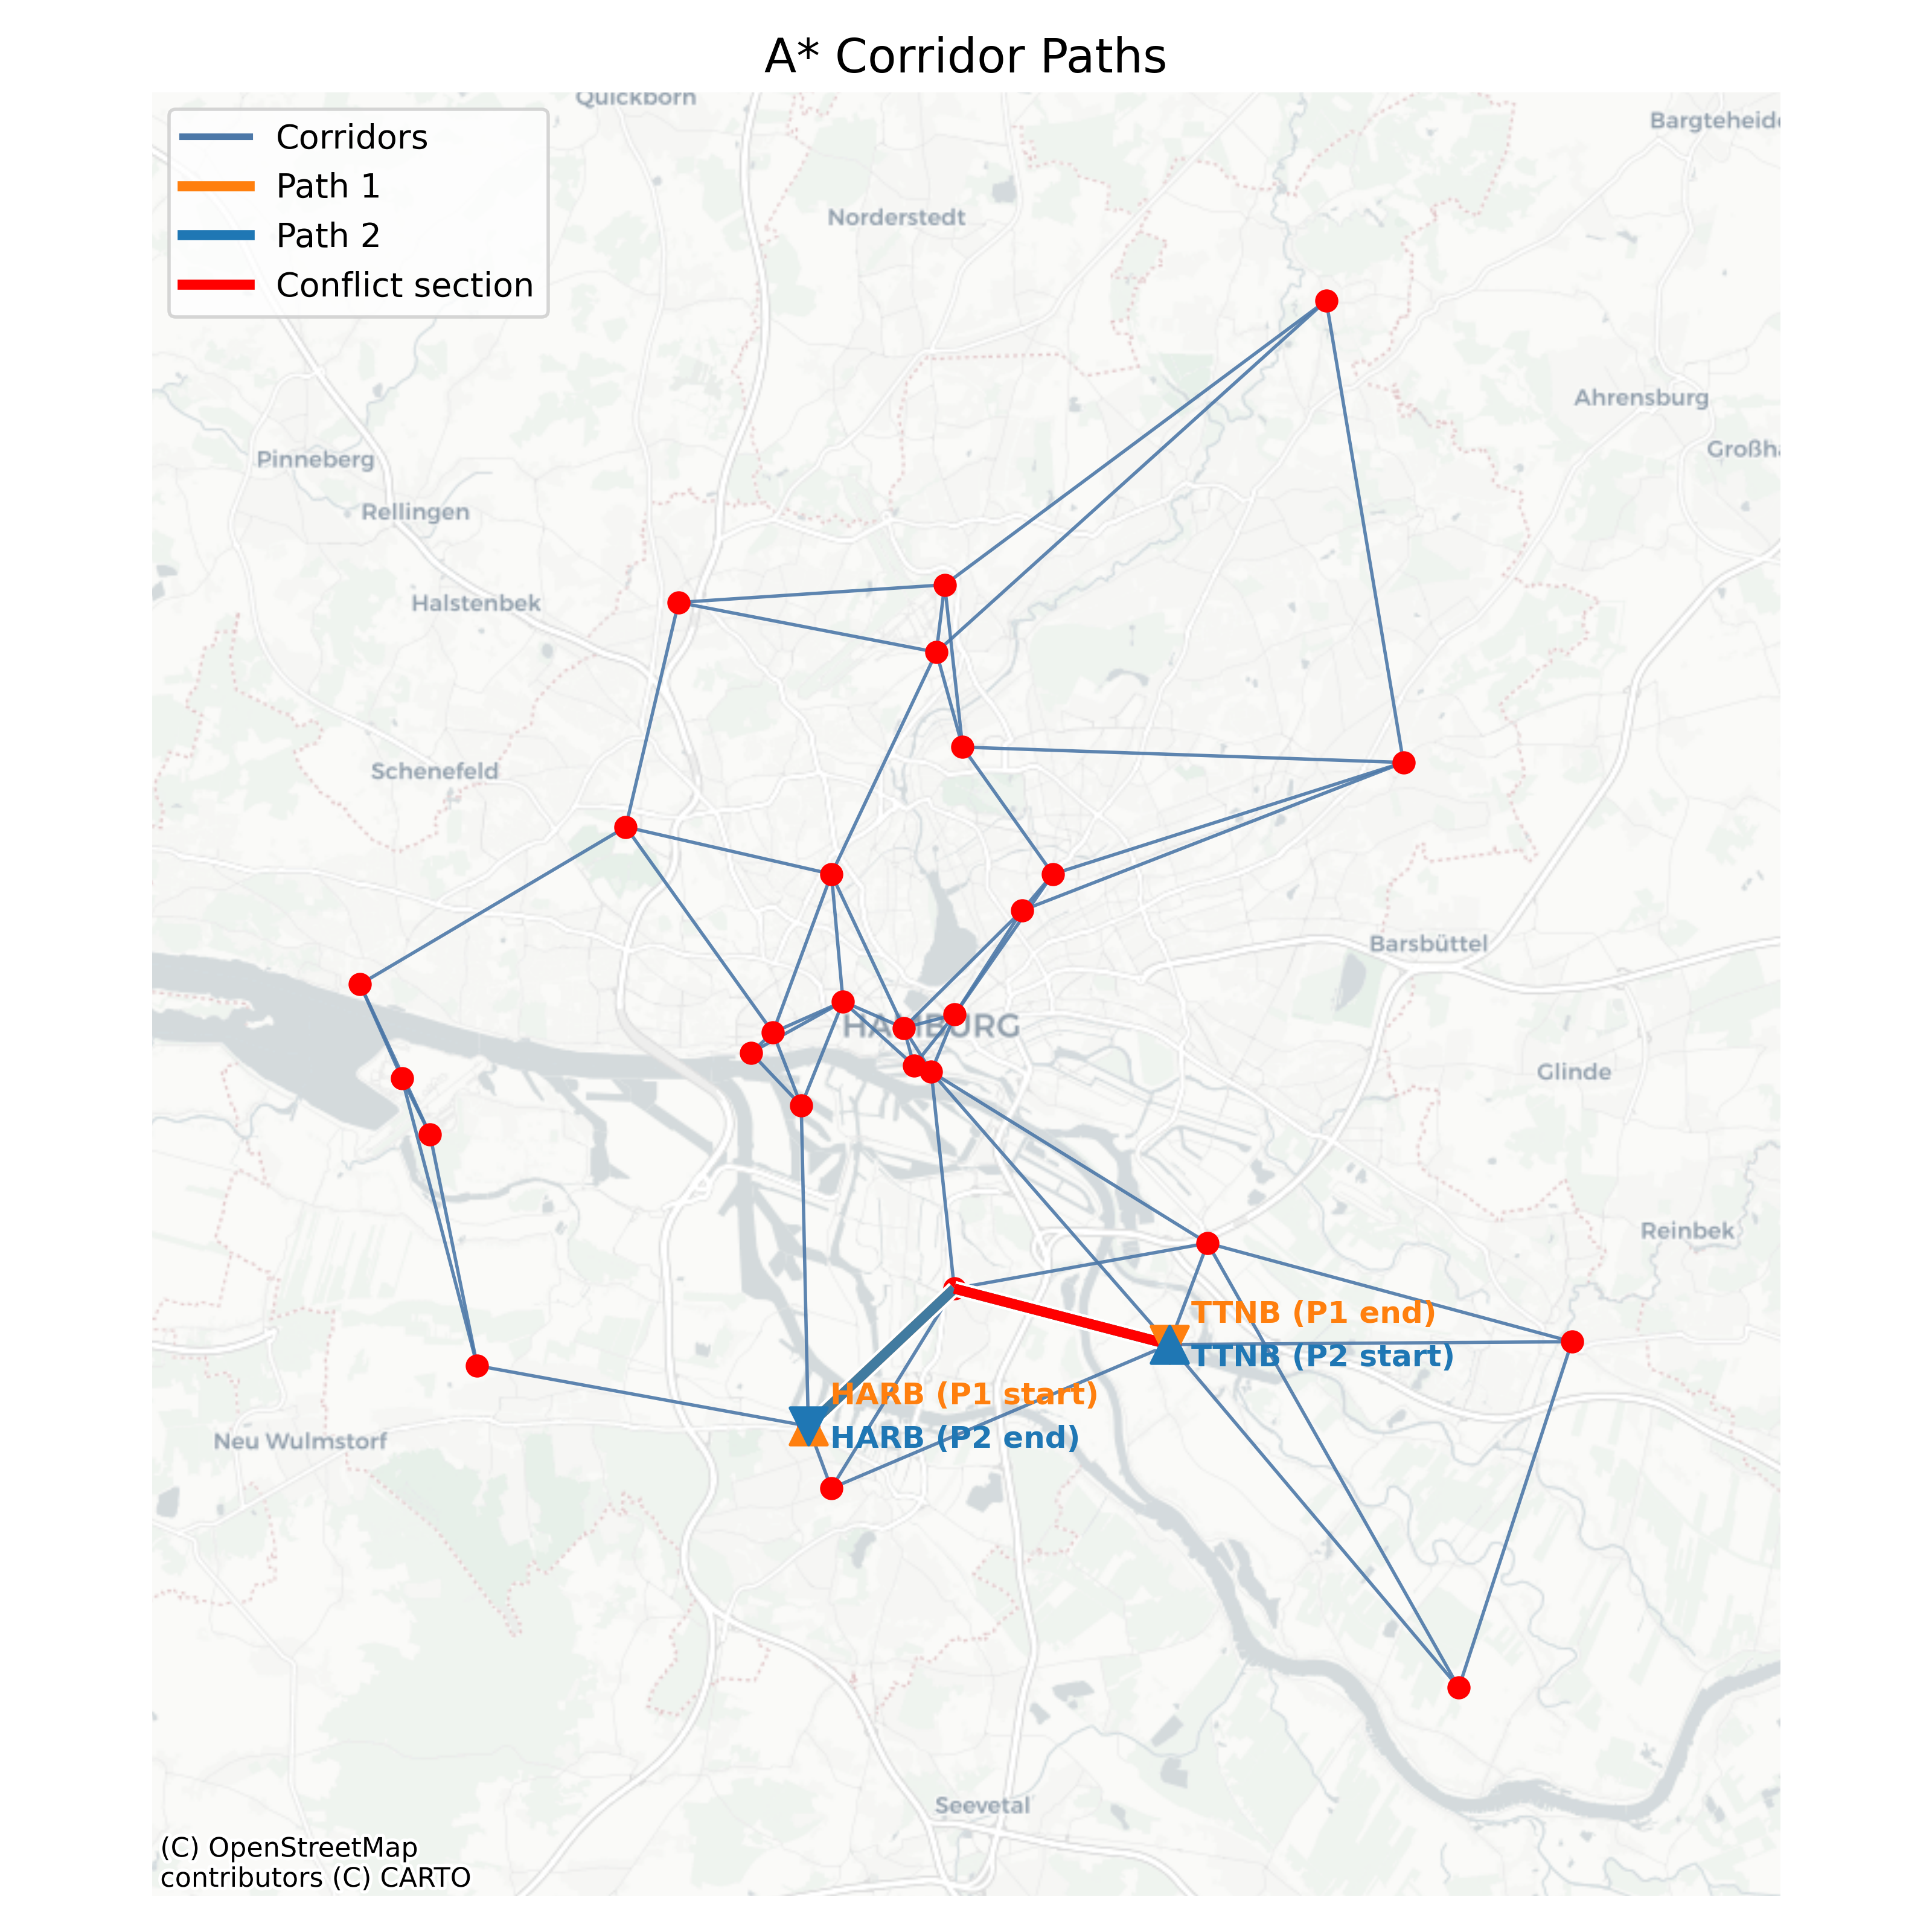
\includegraphics[width=\textwidth]{results/corridors_multiple_paths_1.png}
    \caption{Initial planned routes for interchanged endpoints: both planned paths overlap completely on the shortest corridor segment (conflict).}
    \label{fig:conflict_interchanged_initial}
  \end{subfigure}
  \hfill
  \begin{subfigure}[t]{0.48\textwidth}
    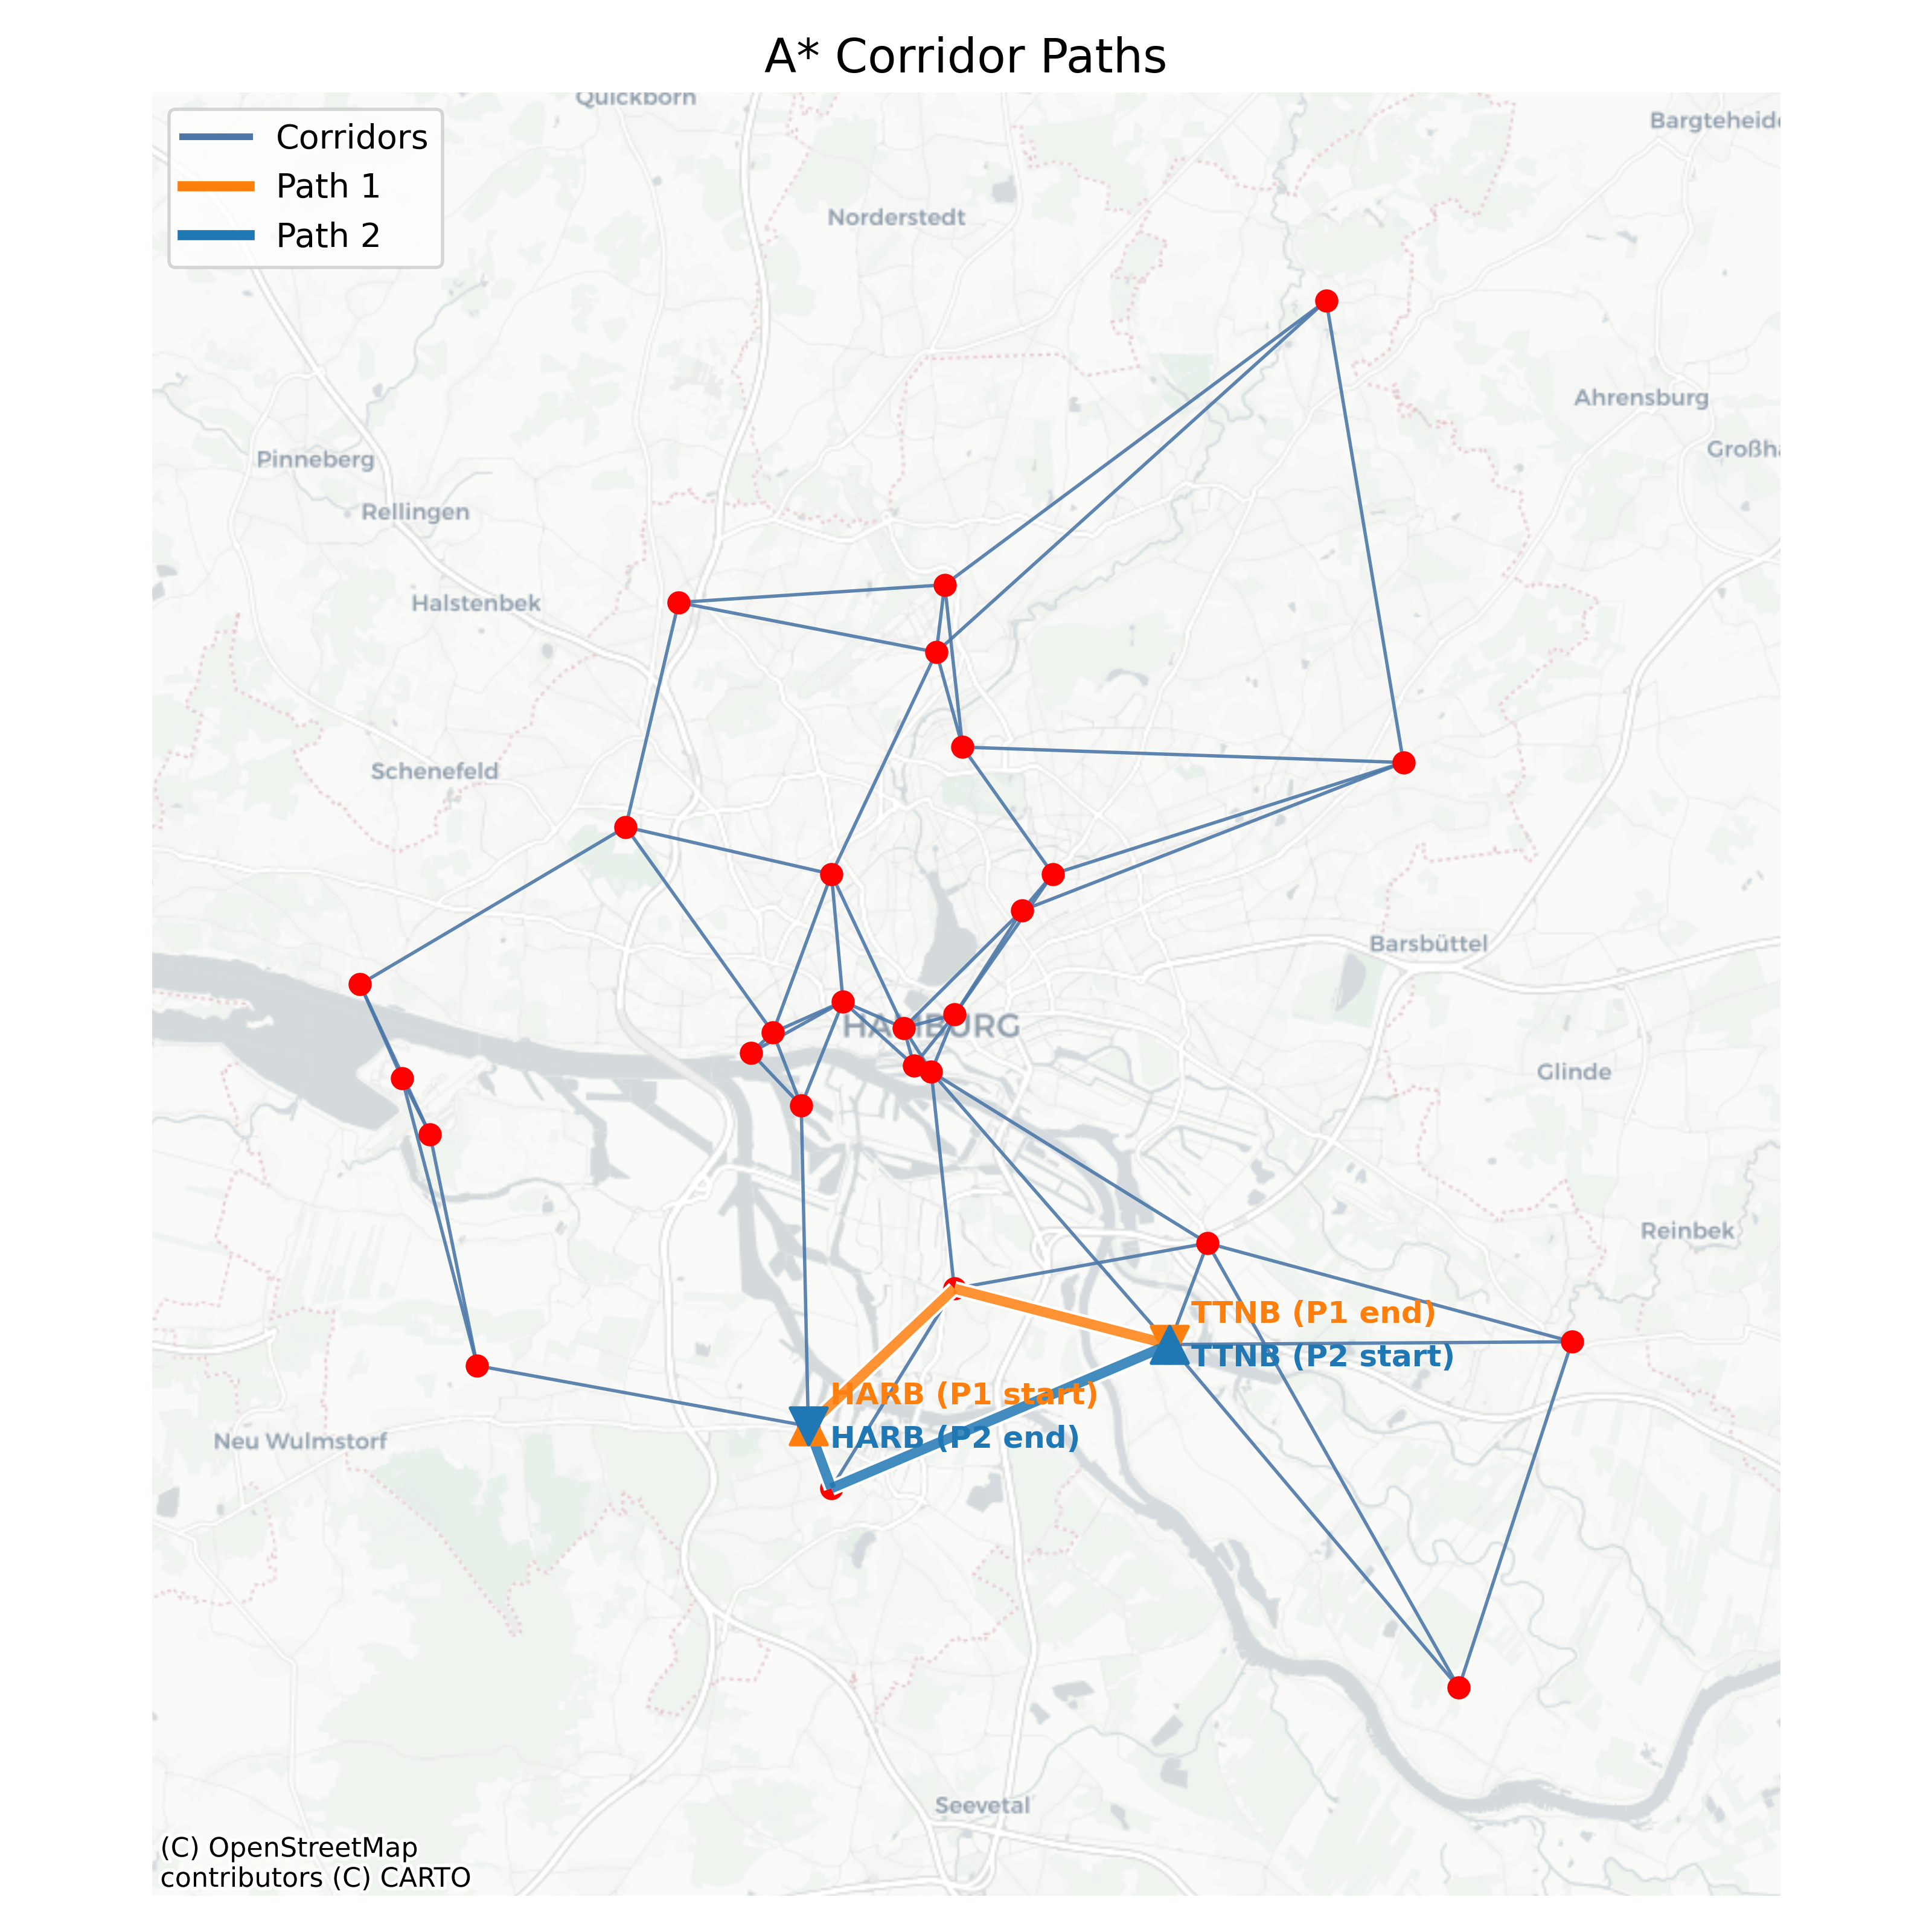
\includegraphics[width=\textwidth]{results/corridors_multiple_paths_resolved_1.png}
    \caption{Re-planned conflict-free route for \texttt{TTNB~$\rightarrow$~HARB} along the second-shortest corridor path, eliminating overlap.}
    \label{fig:conflict_interchanged_resolved}
  \end{subfigure}
  \caption{Conflict handling for interchanged endpoints on planned routes.  
           The later trajectory is re-planned to avoid the overlapping corridor.}
  \label{fig:conflict_interchanged}
\end{figure}

\subsubsection*{Summary}
This case demonstrates the robustness of the rerouting mechanism in situations
where direct shortest paths are infeasible due to complete overlap.
By enforcing the second-shortest path in the graph, the framework maintains
safety while preserving operational feasibility in dense urban networks.

\section{Scalability Evaluation with 100 Trajectories}
\label{sec:scalability_eval}

To assess the computational scalability of the proposed framework, a batch of
100 synchronous trajectory requests was processed. In this setup, each request
was completed before the next one was started. Independent pairs of take-off
and landing vertiports were randomly selected, and successful trajectories were
used for evaluation. Conflict detection and resolution mechanisms were disabled
in this experiment to isolate the baseline computational performance.

\subsection*{Summary Statistics}
The mean and standard deviation of the measured runtimes across the 100 test cases are summarized in Table~\ref{tab:runtime_100}. 
The 100 cases used distinct pairs of take-off and landing vertiports within the Hamburg vertiport network employed in this study, whose corridor graph was fully connected. Because conflict resolution was disabled for this evaluation and the graph connectivity guaranteed a path between any pair, all 100 planned trajectories were successfully generated.

\begin{table}[H]
  \centering
  \caption{Runtime summary over 100 synchronous trajectory requests.}
  \label{tab:runtime_100}
  \begin{tabular}{l r r}
    \toprule
    Metric & Mean (ms) & Std (ms) \\
    \midrule
    Total time              & 162.92 & 38.38 \\
    Trajectory generation   & 151.43 & 38.06 \\
    A* path finding         & 0.41   & 1.21  \\
    \bottomrule
  \end{tabular}
\end{table}

\subsection*{Scatter Plot Analysis}
Figure~\ref{fig:astar_vs_nodes} shows the relationship between A* runtime and \emph{path nodes (count)}. 
No meaningful correlation was observed (e.g., $r\approx0.02$), confirming that A* search latency is essentially independent of the number of nodes traversed.  
In contrast, Fig.~\ref{fig:trajgen_vs_nodes} demonstrates a strong positive correlation (e.g., $r\approx0.75$) 
between \emph{path nodes (count)} and trajectory generation time, consistent with the generator’s per-segment workload.

\begin{figure}[H]
  \centering
  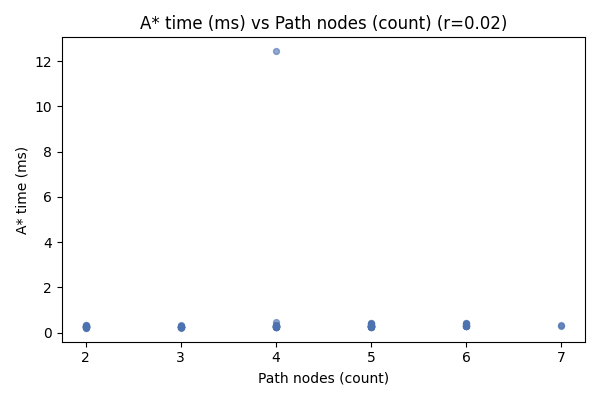
\includegraphics[width=0.7\textwidth]{results/scatter_astar_vs_nodes.png}
  \caption{A* runtime vs.~path nodes (count). Example correlation: $r\approx0.02$.}
  \label{fig:astar_vs_nodes}
\end{figure}

\begin{figure}[H]
  \centering
  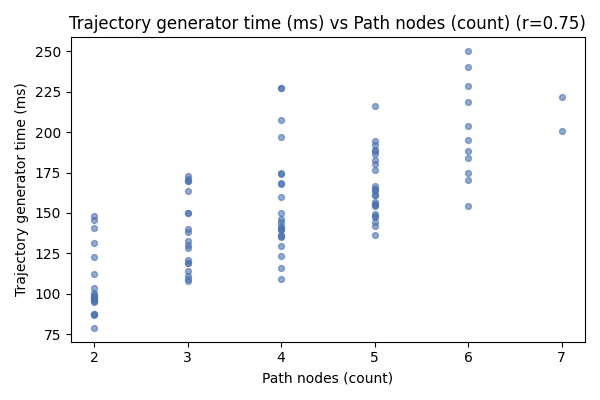
\includegraphics[width=0.7\textwidth]{results/scatter_traj_generator_vs_nodes.png}
  \caption{Trajectory generator runtime vs.~path nodes (count). Example correlation: $r\approx0.75$.}
  \label{fig:trajgen_vs_nodes}
\end{figure}

\subsection*{Runtime Distributions}
The distribution of total processing time across the 100 runs is shown in
Fig.~\ref{fig:hist_total}, with values concentrated in the \SIrange{120}{260}{ms} range. 
The distribution of trajectory generation runtimes (Fig.~\ref{fig:hist_trajgen})
shows a similar pattern, confirming that trajectory generation is the dominant
contributor to total latency.

\begin{figure}[H]
  \centering
  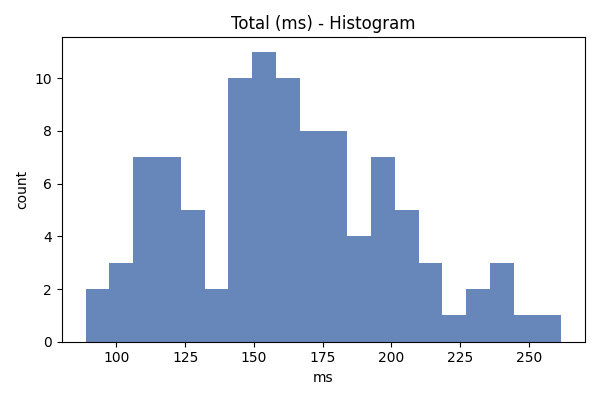
\includegraphics[width=0.7\textwidth]{results/dist_total_ms.png}
  \caption{Histogram of total runtime per trajectory request.}
  \label{fig:hist_total}
\end{figure}

\begin{figure}[H]
  \centering
  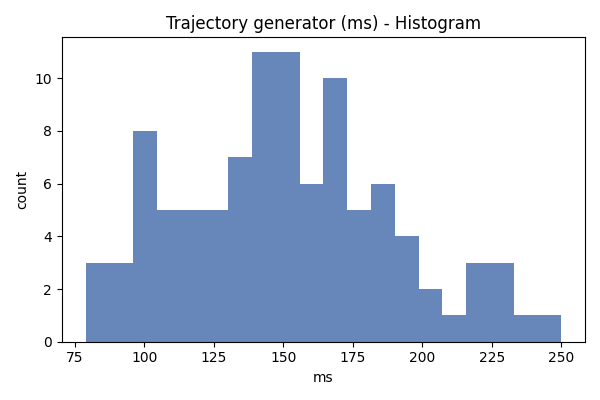
\includegraphics[width=0.7\textwidth]{results/dist_traj_generator_ms.png}
  \caption{Histogram of trajectory generation runtime per request.}
  \label{fig:hist_trajgen}
\end{figure}

\subsection*{Discussion}
These results demonstrate that the A* stage contributes negligibly to total latency,
with mean runtimes well below \SI{1}{ms} across the sampled path sizes. In contrast,
trajectory generation dominates the runtime and increases with the number of path
nodes (and thus legs to synthesize).  
Overall processing times of roughly \SI{160}{ms} per request indicate that the framework
can support real-time urban air mobility (UAM) trajectory planning in a synchronous,
single-request setting. Scaling to parallel, high-volume scenarios will require further
evaluation under active conflict detection and resolution.


\section{Evaluation under Active Conflict Resolution}
\label{sec:results_conflict_eval}

In addition to the synchronous evaluation without conflict detection and resolution (Sec.~\ref{sec:scalability_eval}), 
the framework was further assessed under active conflict handling. 
Fifteen random takeoff–landing pairs were selected from the Hamburg corridor network. 
For each path request, the conflict detection module (Sec.~\ref{sec:ndmap}) and the lateral re-routing strategy (Sec.~\ref{sec:results_conflicts}) 
were engaged. This setup allows measuring the combined latency of A* search, trajectory generation, and any re-planning iterations 
required to produce a conflict-free trajectory.

\subsection{Processing Strategy}
All 15 trajectory requests were processed synchronously, i.e.\ each request was completed 
before the next one started. This mode isolates the latency of the path-planning pipeline 
without concurrent scheduling effects. If NDMap detected a conflict, the edges involved 
were penalized and A* was re-run (Sec.~\ref{sec:results_conflicts}), which may yield 
longer paths and increased runtimes. Two cases could not be resolved by lateral re-routing alone and remained in conflict, 
indicating that an alternative strategy (e.g.\ altitude change or departure delay) would be necessary.

\subsection{Timing Results}
Across the 13 successfully resolved trajectories, the total end-to-end latency 
(from path request to final 4D trajectory) exhibited a wide spread:
\begin{itemize}
  \item \textbf{Count:} 13 trajectories,
  \item \textbf{Mean total time:} \SI{5286.19}{ms},
  \item \textbf{Standard deviation:} \SI{8003.16}{ms}.
\end{itemize}
Two effects plausibly contribute to this variance: (i) the statistics are based on a small sample (\(n=13\)), which makes the estimate of dispersion sensitive to a few long-running cases; and (ii) part of the measured duration includes inter-service I/O overhead, since trajectory samples are exchanged via intermediate files rather than through an in-process interface.

Figure~\ref{fig:conflict_eval_scatter} shows the scatter plot of total time versus 
path distance for these trajectories. A positive correlation \(r=0.76\) indicates that 
longer paths tend to require more processing time, reflecting both increased 
trajectory-generation cost and additional A* iterations in some cases.

\begin{figure}[H]
  \centering
  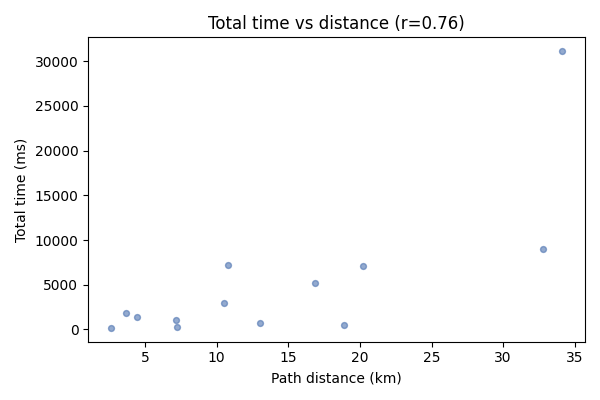
\includegraphics[width=0.48\textwidth]{results/scatter_total_vs_distance_conflicts.png}
  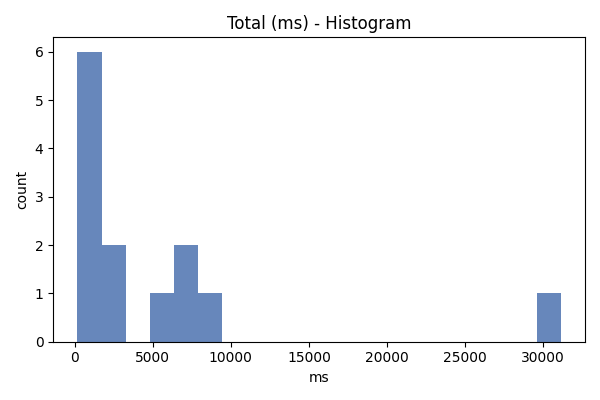
\includegraphics[width=0.48\textwidth]{results/dist_total_ms_conflicts.png}
  \caption{Left: total processing time versus path distance for 13 conflict-free planned trajectories.
           Right: histogram of total processing times across the same runs.}
  \label{fig:conflict_eval_scatter}
\end{figure}

\subsection{Discussion}
Compared to the evaluation without conflict resolution (Sec.~\ref{sec:scalability_eval}), 
both the mean latency and its variance are markedly higher under active conflict handling. 
This is expected, as each detected conflict triggers additional A* searches with modified 
edge weights (Sec.~\ref{sec:results_conflicts}), potentially increasing path length 
and computation time. The two unresolved cases underscore the need for 
more flexible resolution mechanisms—such as altitude assignment, departure delay, or 
risk-map based edge re-weighting—to handle complex conflicts where lateral re-routing alone 
cannot find a feasible solution.

\medskip
\noindent
This evaluation thus highlights the trade-off between safety and responsiveness: 
while lateral re-routing enables automatic deconfliction in many scenarios, 
its runtime cost scales with graph complexity and the number of iterations required.
The observed variance is further influenced by the small sample size and by the current file-based exchange between services; tighter in-process coupling (e.g., integrating CFMS into the planner) would plausibly reduce such overhead.

